
\chapter{Cumulative Surface Deformation over the Permian Basin with Automated Outlier Removal}
\label{CHAP:4-GRL}

%In this chapter,  we present a simple yet effective time series method for creating cumulative surface deformation maps over large regions with severe tropospheric noise. We use the method to create yearly deformation maps over the oil-producing region of the Permian Basin. The method incorporates an automated outlier detection and removal algorithm, which enabled ~2 mm/year agreement with GPS measurements in the presence of $\sim$15 cm of tropospheric noise.


Previous InSAR studies have demonstrated the utility of surface deformation data for understanding causes of induced seismicity; however, these studies focused on study areas $ \sim $ 60-by-60 km or smaller. 
%Basin-wide InSAR surface deformation data with detailed uncertainty quantification are needed for assessing the likelihood of induced seismicity risk in the Permian Basin. 
Since InSAR tropospheric noise variance increases with the distance away from the reference point, it is difficult to expand the InSAR spatial coverage to the entire Permian Basin while retaining millimeter level accuracy.  
In this chapter, we present a time series method for creating large cumulative surface deformation maps over areas containing severe tropospheric noise. 
We developed an outlier detection algorithm that removes InSAR measurements corrupted by severe tropospheric noise (e.g. storms and heat waves).
% withing multiple subsets of interferograms and produces a linear velocity estimate for each subset.
The method reduces the uncertainty in our linear deformation estimates by a factor of 2, down to 1-3 mm/year across the basin. Our results were validated by independent GPS measurements recorded at 13 permanent ground stations. 
We use the method to create yearly deformation maps from November 2014 through January 2019 over the oil-producing region of the Permian Basin, which are available through the Center for Integrated Seismicity Research (CISR) for the broader scientific community. 



%Within Texas, \cite{Shirzaei2016SurfaceUpliftTime} reported indications of surface uplift due to wastewater injection near a 2012 M4.8 earthquake, though limited validation for the ALOS data was available at this site near Timpson, TX \citep{Semple2017IncompleteInventorySuspected}. \cite{Kim2018AssociationLocalizedGeohazards} detected multiple deformation bowls within the Delaware Basin related to wastewater injection, $CO_2$ injection, and hydrocarbon production using Sentinel-1 InSAR data. \cite{Zheng2019WastewaterLeakageWest} incorporated InSAR-derived surface deformation data into a poroelastic model to analyze the geomechanical processes near an uplift signal in northern West Texas. They discovered that the observed surface deformation was likely caused by injection well leakages, rather than pressure increases at the planned injection depth, and the leaks may have contributed to freshwater contamination. More recently, \cite{Deng2020SurfaceDeformationInduced} used ascending Sentinel-1 LOS measurements to infer pore pressure change and Coulomb failure stress change at three sites in the southern Delaware Basin. They suggested that certain groups of earthquakes are likely induced by fluid injection, but noted that local rock structure and media properties are key controls on the area's susceptibility to induced seismicity.

%Previous InSAR studies demonstrated the use of InSAR surface deformation data for understanding causes of induced seismicity; however, these studies only focused on study areas $ \sim $ 60-by-60km or smaller, and basin-wide InSAR surface deformation data with detailed uncertainty quantification are needed for assessing the likelihood of induced seismicity risk. Since InSAR tropospheric noise variance increases with the distance away from the reference point \citep{Emardson2003NeutralAtmosphericDelay}, it is difficult to expand the InSAR spatial coverage to the entire Permian basin while retaining millimeter level accuracy. 

%In this chapter, we show that the increasing quantity and quality of Sentinel-1 SAR data allows us to average thousands of interferograms and mitigate strong tropospheric noise. We developed an outlier detection algorithm that removes InSAR measurements corrupted by severe tropospheric noise (e.g. storms and heat waves) and reduces InSAR measurement uncertainty by another factor of 2, down to 1-3 mm/year across the basin. Our results were validated by independent GPS measurements recorded at 13 permanent ground stations. 
%The InSAR-observed subsidence patterns over the Pecos area can be modeled as dip-slip over multiple normal faults and discretized cylindrical reservoir compaction. 
%Our InSAR deformation maps are now available through the Center for Integrated Seismicity Research (CISR) for the broader scientific community. 
%This dataset, when combined with physics-based reservoir and fault modeling, can produce insights into the causes of induced seismicity. 
%Furthermore, these surface deformation data products can be used to assess the areal effectiveness of the oil and gas production, a measure for estimating which regions of a reservoir are being depleted most quickly. InSAR techniques now provide a low-cost method to assist oil and gas operations and risk management at a basin-scale.

\section{Algorithms}

%In this study, used the Sentinel-1 interferograms from Path 78 and Path 85 processed as described in Section \ref{sec:ch2-insar-processing}.
%We solved for the average LOS velocities over three periods of interest: Nov. 2014 to Jan. 2017, Nov. 2014 to Jan. 2018, and Nov. 2014 to Jan. 2019. Over each time period $T_j$, we computed the cumulative LOS surface deformation as the product of $v_{avg,j}$ and $T_j$. We also solved for the vertical and eastward deformation in the region where Path 78 and 85 overlap (see Section \ref{sec:ch2-insar-decomp}) using the LOS unit vector at each pixel location Figure \ref{fig:los-map})) in the LOS decomposition.


\subsection{Stacking and InSAR time series analysis}
\label{sec:ch4-method-compare}
%[Method only, define equations and formulas. This already outlines how we solve for deformation]

To investigate how InSAR measurement noise influences the line-of-sight (LOS) deformation solutions, we compared the results derived from (1) the stacking method, (2) an SBAS linear deformation (constant velocity) model with $L_1$ and $L_2$-norm penalty functions, and (3) unregularized and regularized SBAS deformation time series. 
We assume there are $M$ small-baseline interferograms that were generated from $N$ SAR scenes acquired over a period of interest. 
We employed a stacking approach \citep{Sandwell1998PhaseGradientApproach} to calculate the average LOS velocity $v_{avg}$ of each ground pixel over a time period of interest $T$ as:
\begin{equation}
%	v_{avg} = \frac{ \sum_{i \in G} \bm{\Delta  d}_i}{\sum_{i \in G} \bm{\Delta t}_i}
	v_{avg} = \frac{\lambda }{4 \pi}  \frac{ \sum_{i \in G} \bm{\Delta  \phi}_i}{\sum_{i \in G} \bm{\Delta t}_i}
	\label{eq:ch4-stacking}
\end{equation}
where $G$ is a subset of interferograms that were formed using two SAR scenes acquired within the time period $T$, and the factor $ \frac{4 \pi}{\lambda} $ converts radians to centimeters. The LOS measurement (in radians) and the temporal baseline of the $i$th interferogram in $G$ are written as $  \bm{\Delta  \phi}_i $ and $ \bm{\Delta t}_i $ respectively. 

Similarly, the SBAS method outlined in Section \ref{sec:ch2-insar-ts} can be augmented with a linear deformation model.
In this formulation, we solve for the average velocity $ v_{avg} $ over this period at each pixel of interest as \citep{Berardino2002NewAlgorithmSurface}:
\begin{equation}
		v_{avg} = \frac{\lambda }{4 \pi} \cdot \arg \min_{v_{avg}} \norm{ \bm{BP} v_{avg} - \bm{\Delta \phi}   }_p
%		\arg \min_{v_{avg}} \norm{ \bm{BP} v_{avg} - \bm{\Delta d}   }_p
	\label{eq:ch4-sbas-linear}
\end{equation}
where $ \bm{B }$ is the $ M \times (N-1) $ SBAS matrix, $ \bm{P}$ is an $ (N-1) \times 1 $ vector of ones, 
%$ \bm{\Delta d} $ is the $ M \times 1 $ vector of LOS measurements (in cm) at this pixel, 
$ \bm{\Delta \phi} $ is the $ M \times 1 $ vector of LOS measurements at this pixel, 
and $ p \in \{1, 2\} $ is the norm used to penalize the data misfit. The $L_2$ linear deformation solution is comparable to the stacking solution (with an assumption of a constant velocity), and the $L_1$ solution is typically less sensitive to measurement outliers than the $L_2$ solution.

The LOS surface velocities between adjacent SAR acquisitions $ \bm{v} = \left[v_1 , \ldots , v_{N-1} \right]^T $ can be solved as:
\begin{equation}
		\bm{v} = \frac{\lambda }{4 \pi} \cdot \arg \min_{\bm{v} } \norm{ \bm{Bv} - \bm{\Delta \phi}   }^2_2 + \alpha \norm{ \bm{Dv} }^2_2  \label{eq:ch4-sbas}
%	\arg \min_{\bm{v} } \norm{ \bm{Bv} - \bm{\Delta d}   }^2_2 + \alpha \norm{ \bm{Dv} }^2_2  \label{eq:ch4-sbas}
\end{equation}
where $ \bm{D} $ is a $ (N-2) \times (N-1) $ matrix, with $1$ on the main diagonal and $-1$ on the superdiagonal, which approximates the first-order differentiation operator. The first term penalizes the data misfit, the second term is a temporal smoothness constraint, and $ \alpha \in \mathbb{R} $ is the weight between the two terms. When $ \alpha = 0 $, the solution is the unregularized SBAS deformation time series. An additional integration of $\mathbf{v}$ over time yields the LOS deformation time series.



\subsection{Tropospheric noise outlier removal}
\label{sec:ch4-outlier-method}

We examined interferograms at the 13 control locations and discovered that non-Gaussian tails (outliers) are present. For example, LOS measurements of the ascending interferograms at pixels near the GPS station TXMC show a near zero median (-4 mm) and a standard deviation of 3.2 cm (Figure \ref{fig:ch4-outliers} (a)). Due to the absence of substantial deformation signal at this station, the standard deviation of the LOS distribution is a measure of turbulent tropospheric noise.  We found that the median LOS turbulent error is close to zero (no systematic noise bias) at all GPS control stations. The standard deviation of the turbulent noise increases as the square root of the distance from the InSAR reference point (Figure \ref{fig:ch4-outliers} (b)). Furthermore, we compared the LOS turbulent noise distribution observed at each GPS station to a normal distribution using a normal probability plot \citep{Filliben1975ProbabilityPlotCorrelation}. We discovered that non-Gaussian tails (outliers) are present (e.g. Figure \ref{fig:ch4-outliers}(c)) as a result of severe tropospheric noise (e.g. storms or heat waves). 



\begin{figure}
	\centering
	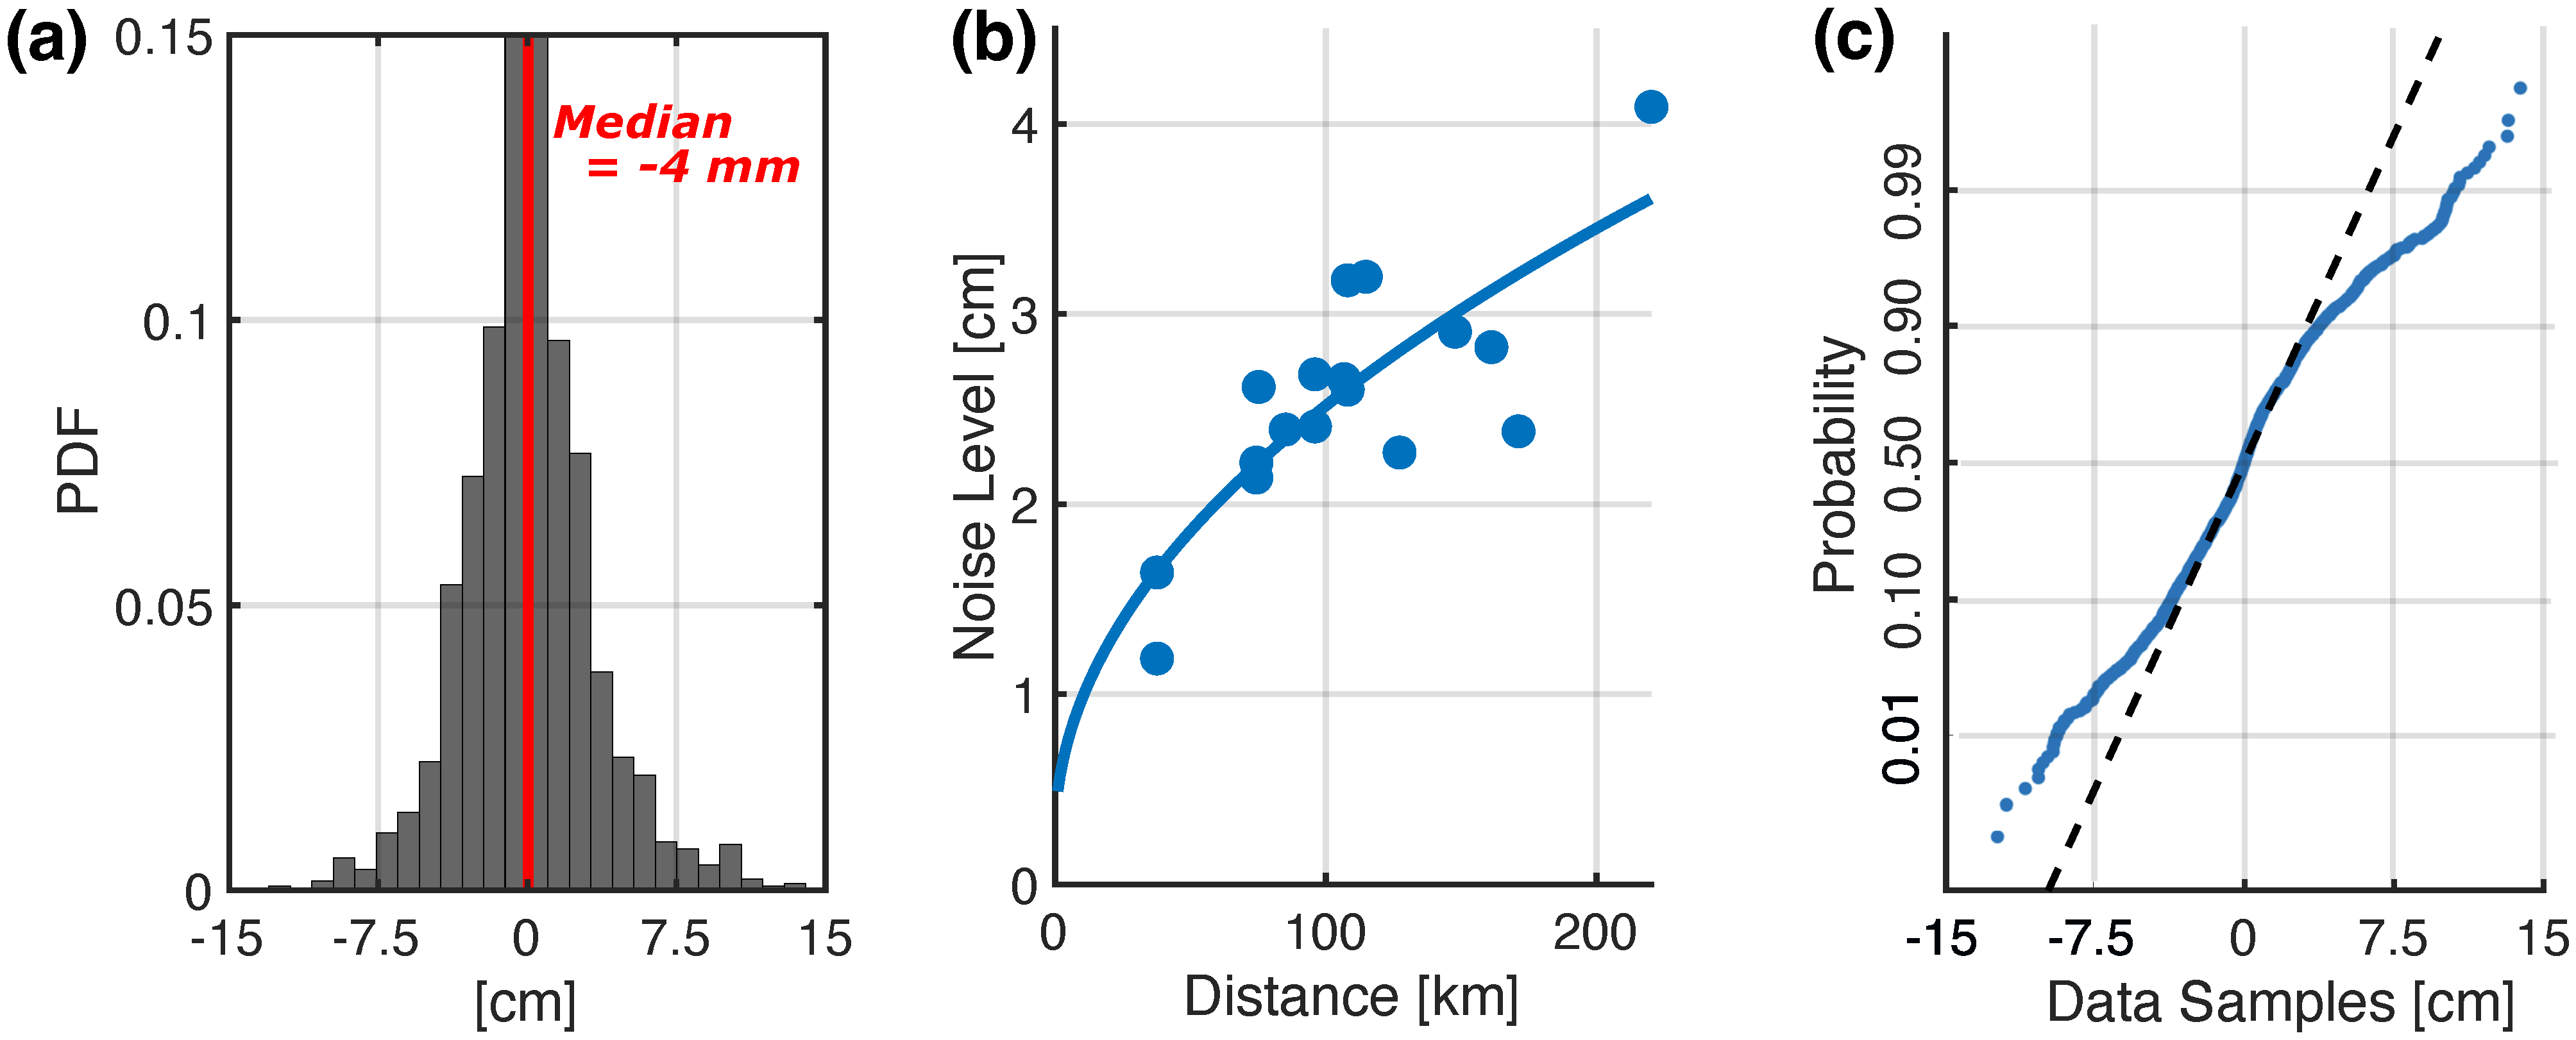
\includegraphics[width=0.99\linewidth]{figures/chapter4-grl/outlier-top-only.pdf}
	%	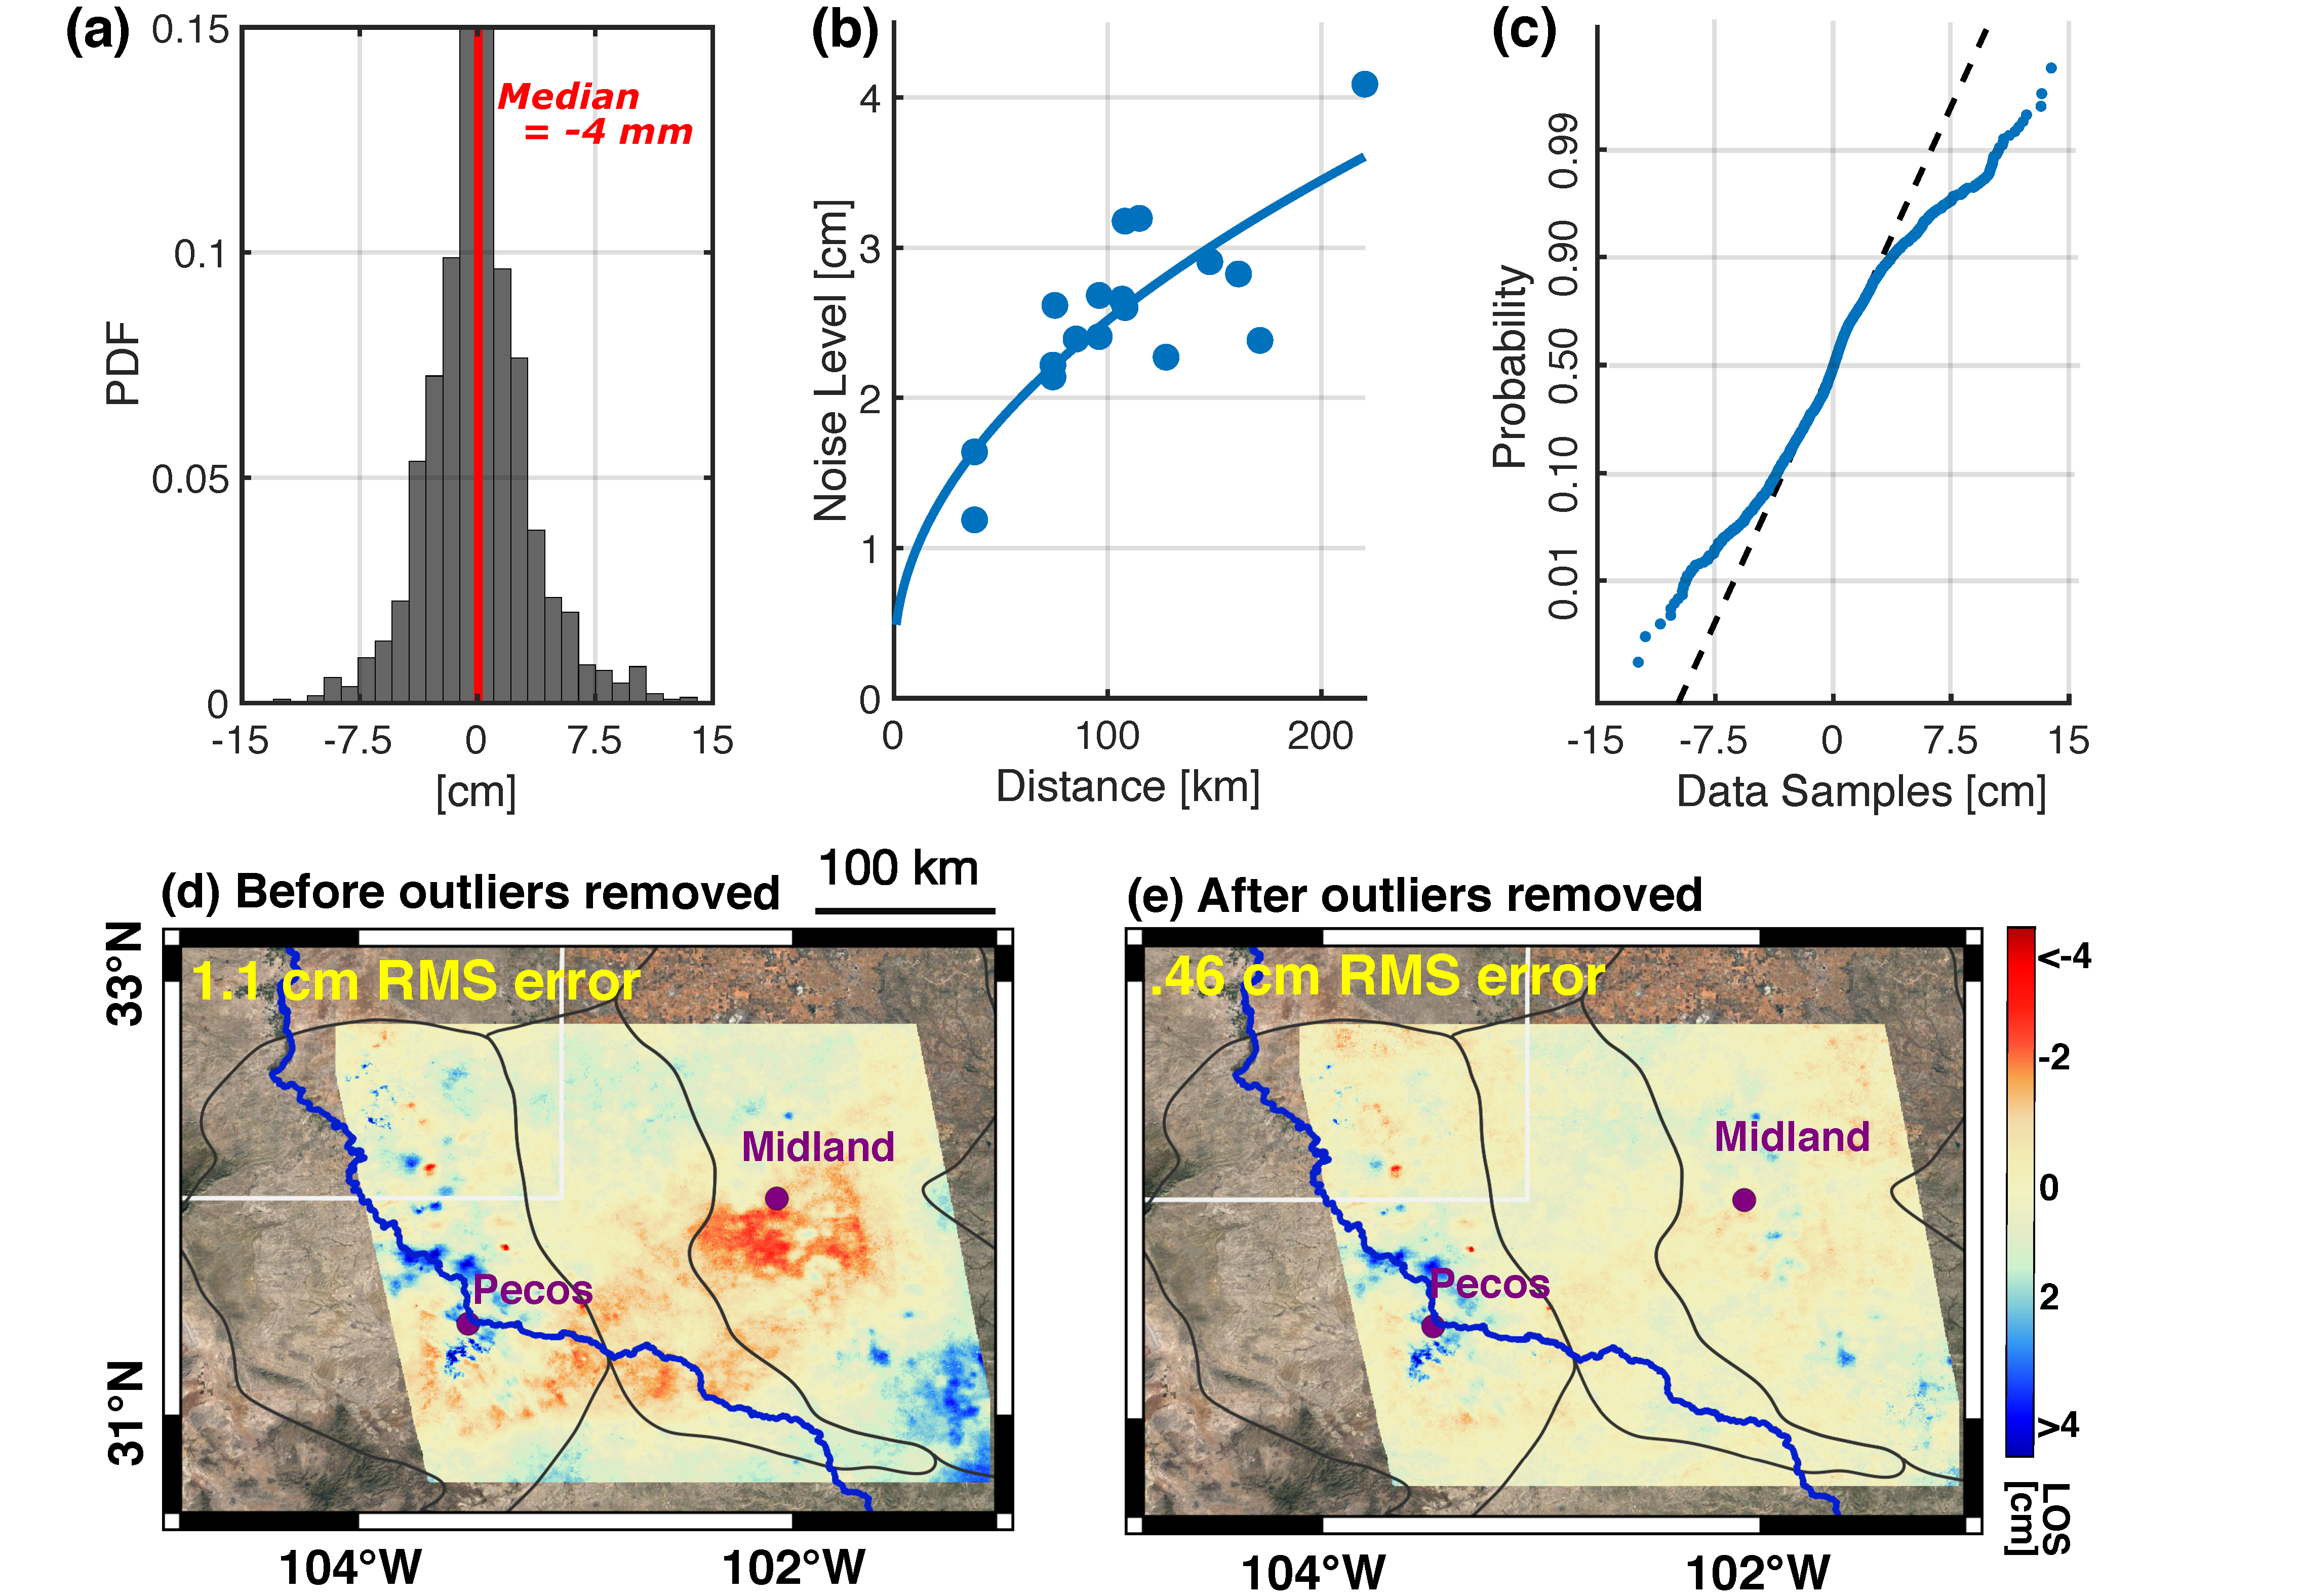
\includegraphics[width=0.95\linewidth]{figures/chapter4-grl/figure2-outlier-removal-5panel.pdf}
	\caption[Noise measurement and tropospheric outliers]{
		(a) LOS measurements (in cm) of all ascending interferograms at the GPS station TXMC. The distribution has a near zero median (-4 mm) and a standard deviation of 3.2 cm. Due to the absence of substantial deformation signals, the standard deviation of the distribution is a measure of LOS turbulent tropospheric noise. (b) The standard deviation of random tropospheric turbulent noise at 13 control locations (blue dots), which increases as the square root of the distance from the InSAR reference point (blue line). (c) A comparison between the tropospheric noise distribution at TXMC with a normal distribution. Dashed line connects the 1st and 3rd quartiles of the data. Troposphere noise following a normal distribution would match the dashed line, and non-Gaussian tails are present. 
	}
	\label{fig:ch4-outliers}
\end{figure}



%When severe tropospheric noise (e.g. storms or heat waves) affects interferograms, the resulting measurement distribution at a given pixel can contain large non-Gaussian tails. 
%Identifying and removing InSAR measurement outliers is crucial for achieving millimeter level accuracy. 
Because severe tropospheric noise may only impact a portion of a SAR image, we identified InSAR measurement outliers at each pixel independently as follows. Given $N$ SAR acquisitions, there are up to $N-1$ InSAR LOS measurements at a pixel of interest that contain the common tropospheric noise of the $k^{th}$ SAR scene. We defined $u_{k,n}$ as the $n^{th}$ such LOS measurement, and $\bar{u}_k$ as the mean absolute measurement:
\begin{equation}
	\bar{u}_k  = \frac{1}{N-1} \sum_{n=1}^{N-1} |u_{k,n}|  
\end{equation}
We labeled $u_{k,n}$ (for all $n$) as outlier measurements if $\bar{u}_k > \mathrm{median}(\mathbf{\bar{u}}) + 4 \sigma_{\mathrm{MAD}}$, where $\mathbf{\bar{u}}=[\bar{u}_1,...,\bar{u}_N]$, and $\sigma_{\mathrm{MAD}}=1.483 \cdot \mathrm{MAD}(\mathbf{\bar{u}})$. Here we employed a robust statistics measure, the median absolute deviation (MAD), for estimating the spread of data samples in the presence of outliers \citep{Hampel1974InfluenceCurveIts, Rousseeuw2011RobustStatisticsOutlier}. Given a vector $\mathbf{x}$ that contains $M$ data samples, $\mathrm{MAD}(\mathbf{x})$ is defined as:
\begin{equation}
	\mathrm{MAD}(\mathbf{x}) =  \underset{m = 1,\ldots M}{\mathrm{median}} \left( \bigr\lvert  x_m - \mathrm{median}(\mathbf{x})  \bigr\rvert \right)
\end{equation}
where $x_m$ is the $m^{th}$ data sample. 



%To account for the large variation in look angle within one Sentinel-1 Interferometric Wide (IW) swath image, we used the LOS unit vector at each pixel location Figure \ref{fig:los-map})) in the LOS decomposition.


\subsection{Line-of-sight Decomposition}
\label{sec:ch4-insar-decomp}


An interferogram measures surface deformation between the two SAR acquisition times along the radar LOS direction. The LOS deformation, $u_{LOS}$, can be written as: 
\begin{align}
	u_{LOS}= \alpha_{e} u_{e} + \alpha_{n} u_{n} + \alpha_{u} u_{u}
\end{align}
where $u_{e}$, $u_{n}$ and $u_{u}$ are the east, north and up displacements, respectively. The radar look vector $\alpha = [\alpha_e, \alpha_n, \alpha_u]$ can be calculated from the known imaging geometry at every pixel location. This varies significantly for Sentinel-1 due to the $ \sim$250 km wide swath (Figure \ref{fig:los-map}). 


\begin{figure}
	\centering
	%	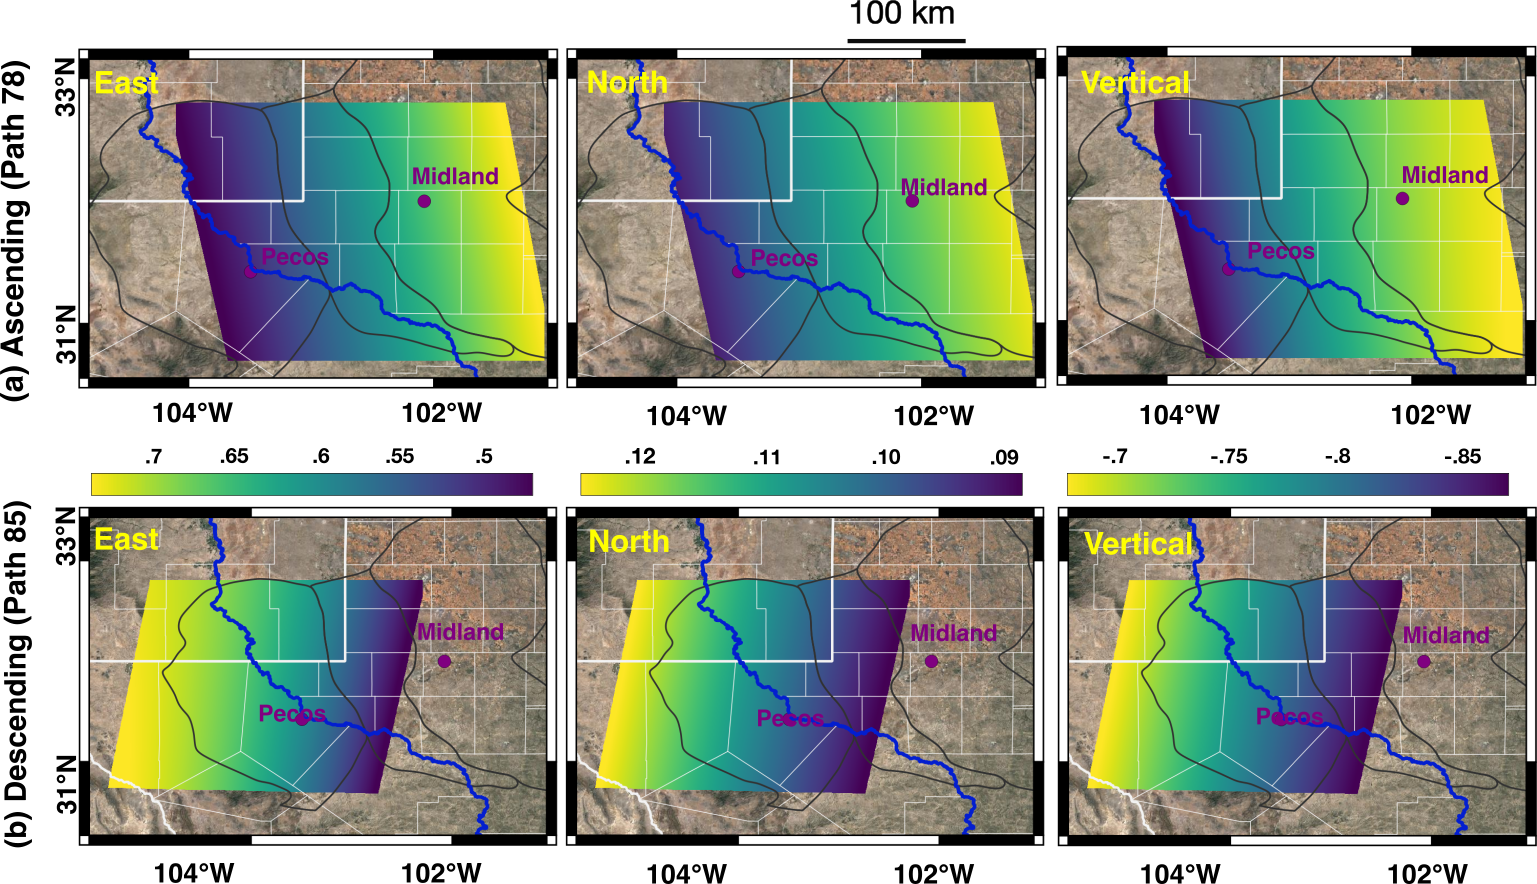
\includegraphics[width=.98\textwidth]{paper1-permian/figures/supplement/figureS2-los.pdf}
	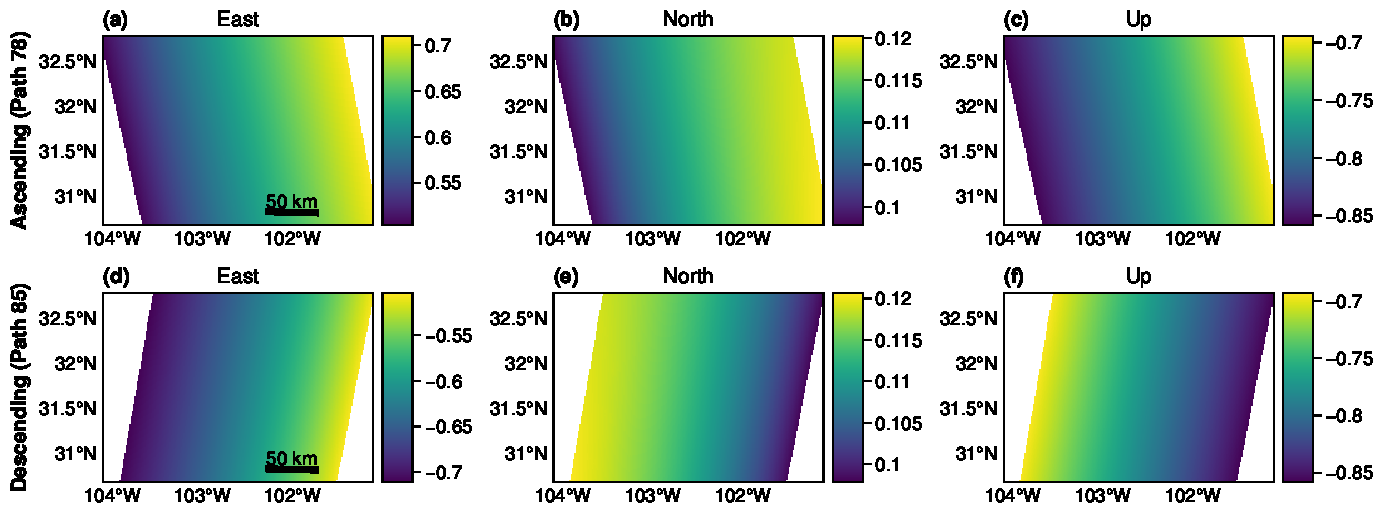
\includegraphics[width=.98\textwidth]{figures/chapter2-sar/figure_los_enu_coeffs.pdf}
	\caption[East, north, and vertical coefficients of Sentinel-1 LOS vectors]{East, north, and vertical coefficient of the LOS unit vector of all Sentinel-1 Path 78 and Path 85 pixels. Positive LOS direction points away from the satellite to the ground.
	}
	\label{fig:los-map}
\end{figure}


In regions where InSAR data are available from two LOS directions, we can decompose the ground motion into its eastward and vertical components.
To perform the decomposition, we first write $u_{asc}$ and $u_{desc}$ in terms of $u_e$, $u_n$ and $u_u$:
\begin{align}
	u_{asc} &= \alpha_{a,e} u_{e} + \alpha_{a,n} u_{n} + \alpha_{a,u} u_{u}\\
	u_{desc} &= \alpha_{d,e} u_{e} + \alpha_{d,n} u_{n} + \alpha_{d,u} u_{u}
\end{align}
We can express $u_e$ and $u_u$ as:
\begin{align}
	u_{e} &\approx  \frac{1}{\beta}  \left[\alpha_{d,u}  u_{asc} - \alpha_{a,u} u_{desc} \right] \\
	u_{u} &\approx  \frac{1}{\beta}  \left[\alpha_{a,e} u_{desc} - \alpha_{d,e}  u_{asc}  \right] 
\end{align}
where  $ \beta = {\alpha_{a,e} \alpha_{d,u}- \alpha_{d,e} \alpha_{a,u}} $.
Because Sentinel-1 satellites are operating in a near-polar orbit, the north look coefficients $\alpha_{a,n}$ and $\alpha_{d,n}$ are both relatively small. Ignoring 1 cm northward motion in $u_n$ only leads to $\sim$ 0.1-0.2 mm error in $u_e$ and $\sim$ 1 mm error in $u_u$ at most locations.  








%\subsection{Uncertainty Propagation through LOS decomposition}
%\label{sec:ch2-decomp-uq-prop}
%Since the LOS decomposition is a linear operation, given two LOS uncertainties, we can use linear uncertainty propagation theory to determine the vertical/horizontal uncertainties.
%
%TODO: move this to appendix or not?




\section{Time series comparisons and outlier removal}
\label{sec:ch4-ts-compare-result}

%- Describe the GPS comparisons for the stacking+outlier results, cutting errors by 2x [Maybe with your uncertainty tables]
%- Bottom half of outlier figure showing the visible artifacts removed
%- Talk about the time series comparison figure, how each had problems, then after outlier removal most converge (+ table quantifying the before/after)
%- conclude all methods converge and we use a simple stacking with outlier removal to calculate cumulative deformation.


Here we used the Sentinel-1 interferograms from Path 78 and Path 85 processed as described in Section \ref{sec:ch3-insar-processing}. 
Using each time series method from Section \ref{sec:ch4-method-compare}, we solved for the cumulative LOS deformation over three periods of interest: Nov. 2014 to Jan. 2017, Nov. 2014 to Jan. 2018, and Nov. 2014 to Jan. 2019. 
For the time series methods calculating an average velocity $v_{avg,j}$ over the $j$th time period $T_j$ , we computed the cumulative LOS surface deformation as the product $v_{avg,j} \cdot T_j$.
%Over each time period 

%We solved for the average LOS velocities over three periods of interest: Nov. 2014 to Jan. 2017, Nov. 2014 to Jan. 2018, and Nov. 2014 to Jan. 2019. Over each time period $T_j$, we computed the cumulative LOS surface deformation as the product of $v_{avg,j}$ and $T_j$. 
%We also solved for the vertical and eastward deformation in the region where Path 78 and 85 overlap (see Section \ref{sec:ch4-insar-decomp}) using the LOS unit vector at each pixel location Figure \ref{fig:los-map})) in the LOS decomposition.

%Little surface deformation occurred between Nov. 2014 and Jan. 2019 at the 13 GPS permanent GPS stations. 
To compare the time series methods, we projected the 13 GPS ENU time series onto the radar LOS. We computed the average GPS LOS velocity with a linear regression and used this as ground truth. 
%We first compared InSAR solutions using the ascending Path 78 data between Nov. 2014 and Jan. 2018.
We found that InSAR tropospheric noise has a strong influence on all the surface deformation solutions before removing the measurement outliers. As an example, Figure \ref{fig:ch4-compare-ts} (a) shows the ascending Path 78 LOS solutions between Nov. 2014 and Jan. 2018 at the GPS station TXSO before removing InSAR measurement outliers. The random tropospheric noise creates up to $\sim$6 cm of error in the unregularized SBAS surface deformation time series. This error can be reduced by increasing $ \alpha$ in Equation \eqref{eq:ch4-sbas}. As $\alpha$ increases, the LOS deformation time series converge to the $L_2$ linear deformation (constant velocity) solution. 



\begin{figure}
	\centering
	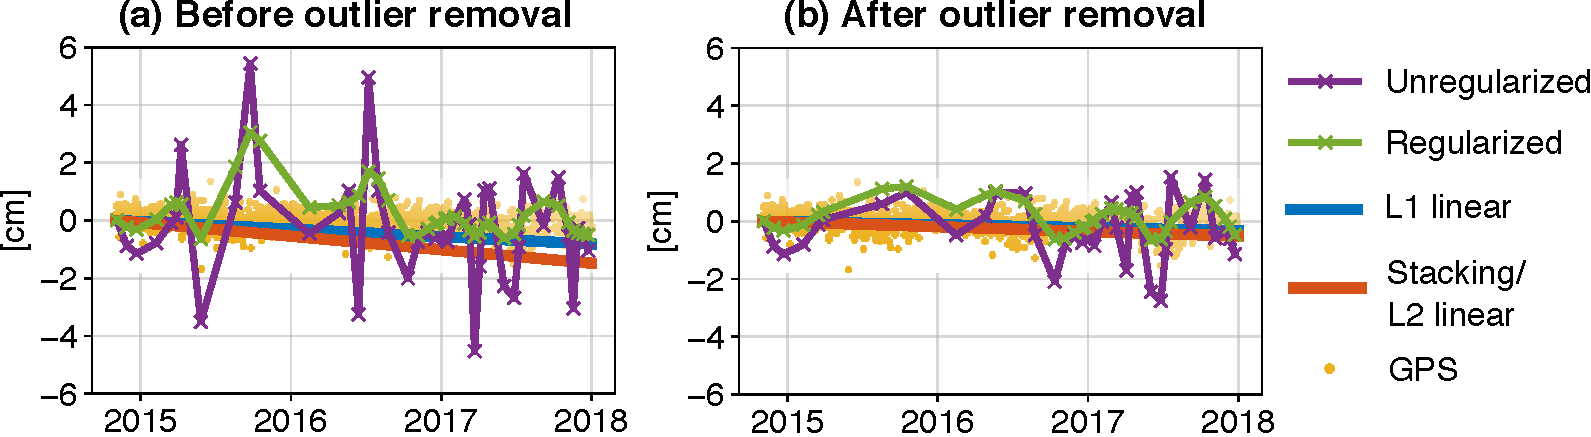
\includegraphics[width=\textwidth]{figures/chapter4-grl/supplement/figureS5-compare-insar-2panel.pdf}
	\caption[Comparisons of InSAR SBAS solutions]{Comparisons of InSAR unregularized SBAS time series (purple), regularized SBAS time series (green), linear deformation trend estimated by minimizing the $L_1$-norm of the residuals (blue), and the $L_2$-norm of the residuals/ stacking approach (red)  (a) before and (b) after removing LOS measurement outliers. ENU GPS data from station TXSO has been projected onto the radar LOS (orange dots).}
	\label{fig:ch4-compare-ts}
\end{figure}

After removing InSAR outlier measurements associated with local weather events, all SBAS time series methods produce more accurate and consistent deformation trends (Figure \ref{fig:ch4-compare-ts} (b)). The unregularized SBAS time series still contains up to $\sim$3 cm of tropospheric noise, which leads to long-wavelength artifacts in the basin-wide deformation maps. The $ L_1 $ and $ L_2 $ linear deformation solutions show close agreement ($<$ 2 mm difference) at all GPS stations. 
% for estimating cumulative surface deformation for all time periods. 
%in the Permian Basin. 
Table \ref{tab:compare-errors} summarizes the differences before and after removing outliers for the four methods using the root mean square (RMS) and the worst-case absolute differences between InSAR and all 13 GPS inferred average LOS velocities.
Since both linear methods suggest a deformation trend consistent with the stacking approach, we chose the simple stacking method as the final processing strategy.

\begin{table}
	\caption{Errors (in mm) in four SBAS ascending LOS deformation (Nov. 2014 - Jan. 2018) solutions}
	\centering
	\begin{tabular}{|c|c|c|}
		\hline 
		& Before the outlier removal & After the outlier removal \\
		& (RMS / Worst) & (RMS / Worst) \\
		\hline
		Unregularized &  22 / 99     &  14 / 43         \\\hline
		Regularized   &    14 / 63   &   10  / 27       \\\hline
		L1 linear deformation          &   7 / 11      & 4 / 8      \\\hline
		L2 linear deformation          &   10 / 22        & 4 / 8      \\\hline
	\end{tabular}
	\label{tab:compare-errors}
\end{table}

We see a striking visual difference in the Path 78 stacking-derived cumulative deformation from Nov. 2014 to Jan. 2018 after removing tropospheric outliers (Figure \ref{fig:ch4-outliers-visual}).
There are cm-level tropospheric artifacts in the cumulative deformation solution that includes all noisy measurements
% by using either $L_1$ or $L_2$ linear deformation models 
(Figure \ref{fig:ch4-outliers-visual}(a)).   
%The presence of InSAR measurement outliers resulted in long-wavelength artifacts ($ \sim $100km and greater) in the cumulative deformation solutions which did not match the GPS station measurements (Figure \ref{fig:ch4-outliers-visual} (a)).
These long wavelength artifacts (e.g. the red streak near Midland) do not match the GPS stations measurements.
However, the artifacts were mitigated using the pixel-wise outlier removal algorithm (Figure \ref{fig:ch4-outliers-visual} (b)). 

\begin{figure}
	\centering
	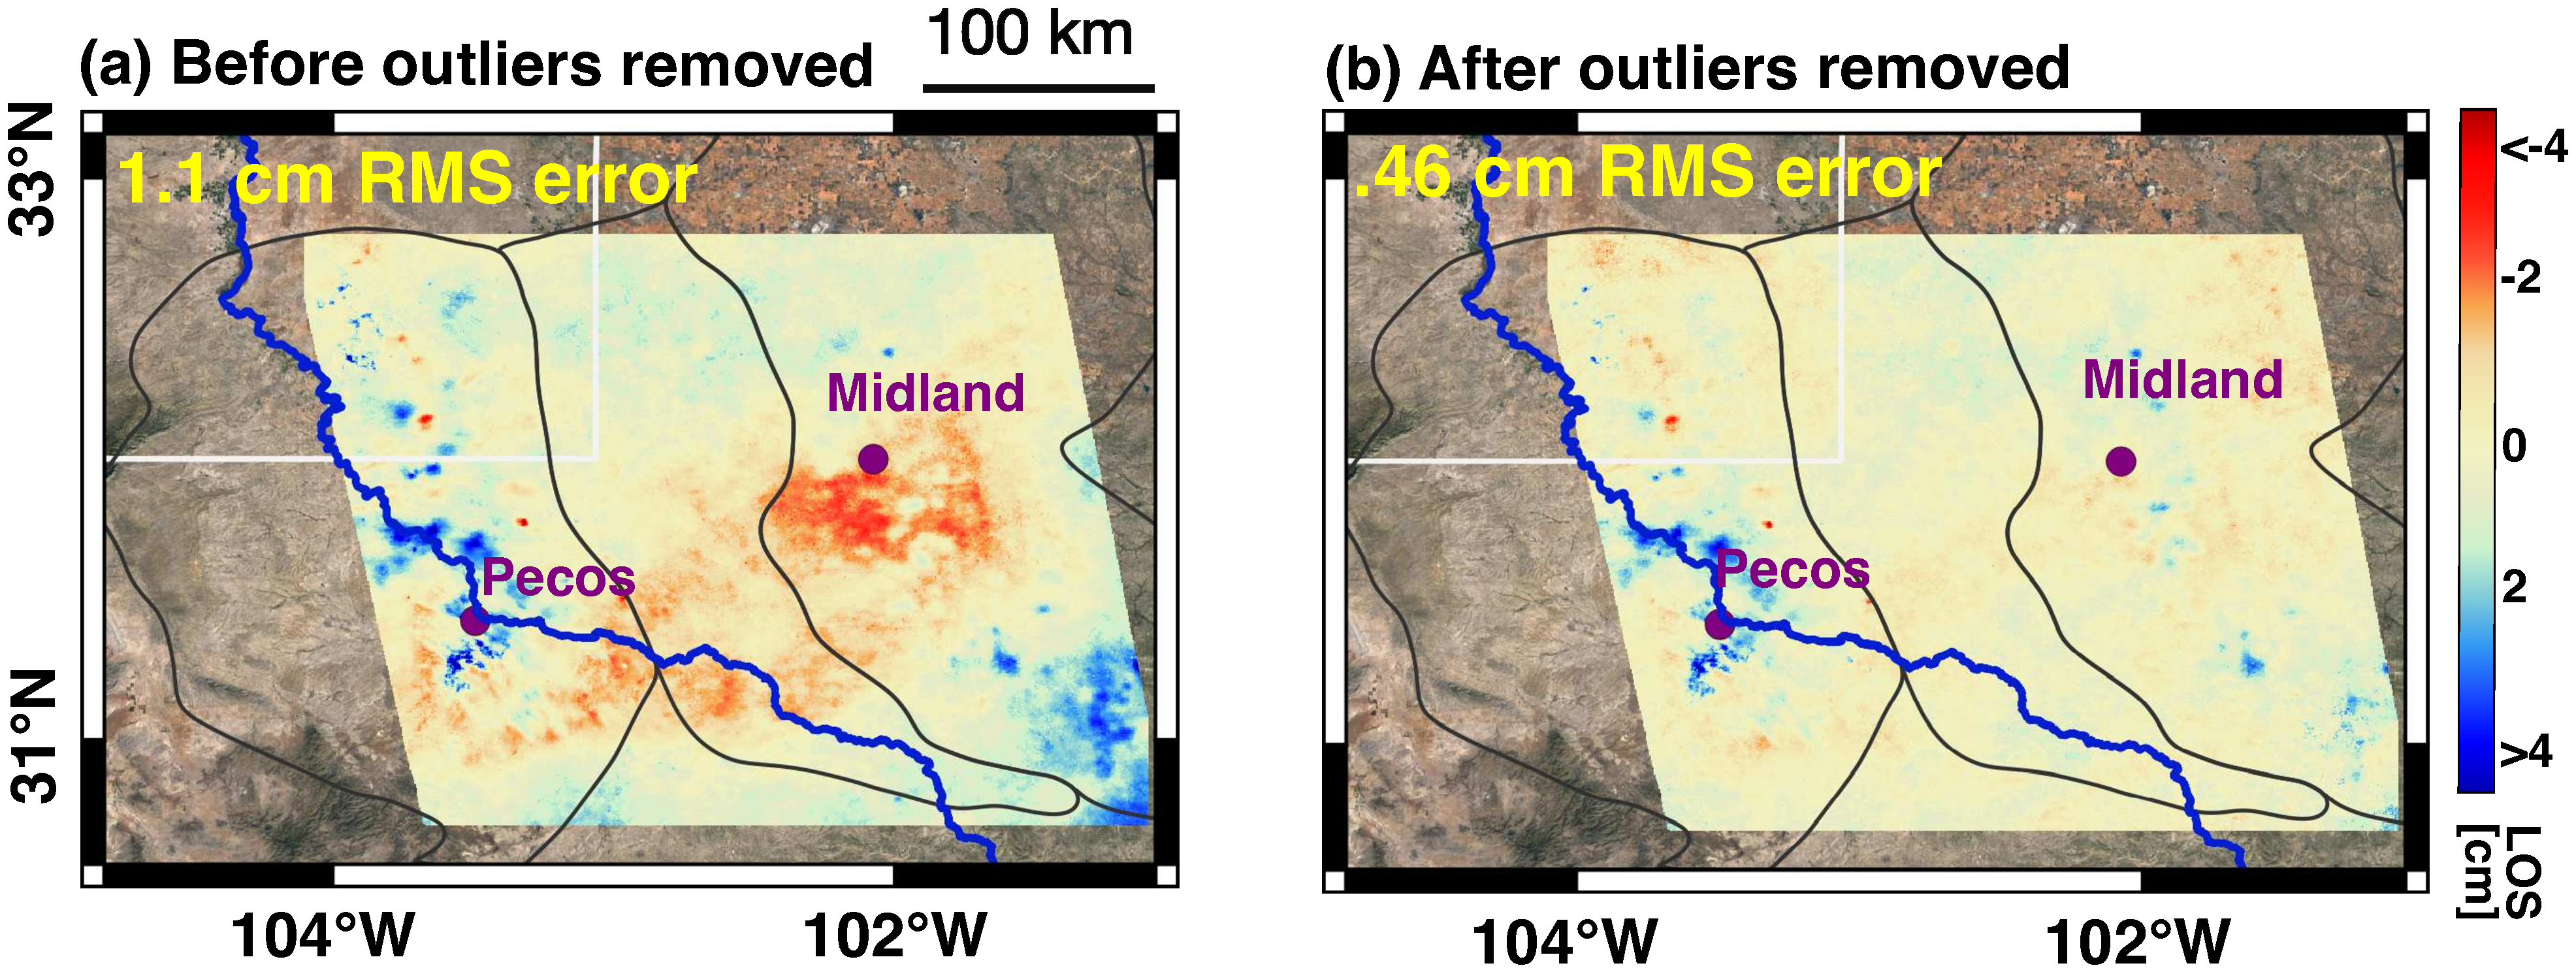
\includegraphics[width=0.99\linewidth]{figures/chapter4-grl/outlier-bottom-only.pdf}
	\caption[Tropospheric outlier removal comparison]{
		Cumulative ascending LOS deformation solutions (Nov. 2014 - Jan. 2018) 
		(a) before and (b) after excluding InSAR outlier measurements. Note that 1.1 cm cumulative error over 3 years is equivalent to 3.5 mm/year RMS error in the velocity estimate.}
	\label{fig:ch4-outliers-visual}
\end{figure}






%We similarly performed 
%We derived the cumulative ...
%the stacking an outlier on X Y Z on Path 85 and compared. table.


%Using the 13 GPS east, north, and up time series as ground truth, we quantified the errors in the InSAR stacking solutions before and after the outlier removal. 
%We summarize the errors in the InSAR stacking solutions before and after the outlier removal for Path 78 and 85 in Tables \ref{tab:gps-error-78} and \ref{tab:gps-error-85}, respectively. 
%There are 13 permanent GPS stations in the ascending SAR footprint.
%At each GPS location, we projected the GPS time series to the radar line-of-sight (LOS), and we computed the GPS-inferred average LOS velocity through a linear regression. 

Table \ref{tab:gps-error-78} shows the RMS and the worst-case absolute differences between the ascending Path 78 InSAR and GPS inferred average LOS velocities for all three study periods. 
For each time period, our outlier removal algorithm reduced the uncertainty in the InSAR stacking solution by a factor of $\sim$2, down to 1-3 mm/year RMS across the basin.
Similarly, there are 5 permanent GPS stations in the descending Path 85 SAR footprint, and Table \ref{tab:gps-error-85} shows the uncertainty in the descending stacking solutions using these stations for comparison.
We see a similar reduction in noise by a factor of $\sim$2 for Path 85.
%Both Table \ref{tab:gps-error-78} and Table \ref{tab:gps-error-85} show that . 
Note that for a given period of interest $T_j$, the LOS velocity error $ E_{vel,j} $  propagates into the cumulative deformation error $ E_{c, j} $ as $ E_{c,j} = E_{vel,j} \cdot T_j $. 
%from Table \ref{tab:gps-error-78} or \ref{tab:gps-error-85}



\begin{table}
	\caption{InSAR ascending Path 78 LOS velocity estimation errors (in mm/year) using the stacking method}
	\centering
	\begin{tabular}{|c|c|c|}
		\hline 
		& Before the outlier removal & After the outlier removal \\
		& (RMS / Worst) & (RMS / Worst) \\
		\hline
		Nov. 2014 - Jan. 2017 & 3.8 / 9.5         & 1.9 / 5.9       \\\hline
		Nov. 2014 - Jan. 2018 & 3.3 / 7.1         & 1.3 / 2.5       \\\hline
		Nov. 2014 - Jan. 2019 & 2.0 / 6.1         & 1.1 / 2.5       \\\hline                
	\end{tabular}
	\label{tab:gps-error-78}
\end{table}

\begin{table}
	\caption{InSAR descending Path 85 LOS velocity estimation errors (in mm/year) using the stacking method}
	\begin{tabular}{|c|c|c|}
		\hline 
		& Before the outlier removal & After the outlier removal \\
		& (RMS / Worst) & (RMS / Worst) \\
		\hline 
		Nov. 2014 - Jan. 2017 & 7.8 / 13.8                            & 2.9 / 5.0                          \\\hline
		Nov. 2014 - Jan. 2018 & 3.7 / 7.5                             & 2.7 / 5.6                          \\\hline
		Nov. 2014 - Jan. 2019 & 1.6 / 2.8                             & 0.8 / 1.6  \\\hline     
	\end{tabular}
	\label{tab:gps-error-85}
\end{table}



%To evaluate the performance of our InSAR processing strategy, 
%We projected GPS data recorded at 13 control stations onto the LOS directions to use as ground truth. The differences between InSAR and GPS inferred average LOS velocities were used as a measure of the uncertainty in the InSAR surface deformation solutions. 
%We found that stacking reduces the impact of random Gaussian turbulent noise by $ \sim \sqrt{N} $, where $ N $ is the number of SAR acquisitions. The outlier removal algorithm further reduces the uncertainty in the LOS velocity estimates by a factor of 2, down to 1-3 mm/year across the basin. For example, the average InSAR velocity along the ascending LOS direction between Nov. 2014 and Jan. 2018 shows a root mean square (RMS) error of 3.4 mm/year before the outlier removal, and 1.5 mm/year after the outlier removal. 

%Additionally, we compared InSAR LOS deformation solutions as derived from (1) the stacking method, (2) a SBAS linear deformation model with $L_1$ and $L_2$-norm penalty functions, and (3) unregularized and regularized SBAS deformation time series (Section \ref{sec:ch4-method-compare}). 
%These InSAR time series algorithms can be implemented using software packages such as Generic InSAR Analysis Toolbox (GIAnT) \citep{Agram2013NewRadarInterferometric}, STAMPS \citep{Hooper2012RecentAdvancesSar}, and LiCSBAS \citep{Morishita2020LicsbasOpenSource}. 
%Removing the detected outliers leads to more accurate and consistent surface deformation solutions in all three cases. 


%We found that stacking reduces the impact of random Gaussian turbulent noise by $ \sim \sqrt{N} $, where $ N $ is the number of SAR acquisitions. The outlier removal algorithm further reduces the uncertainty in the LOS velocity estimates by a factor of 2, down to 1-3 mm/year across the basin. For example, the average InSAR velocity along the ascending LOS direction between Nov. 2014 and Jan. 2018 shows a root mean square (RMS) error of 3.4 mm/year before the outlier removal, and 1.5 mm/year after the outlier removal. 



%
%\subsection{InSAR LOS velocity estimation error}
%\label{sec:error-quant}


\section{Surface deformation in the Permian Basin}



The Sentinel-1 cumulative LOS deformation solutions reveal numerous surface deformation features over the oil-producing region in the Permian Basin (Figure \ref{fig:ch4-insar-los}). From the ascending geometry, we observed no substantial deformation in the Central Basin Platform, where oil and gas are mostly produced from conventional reservoirs. In the Midland and Delaware Basins, we observed an accelerating surface deformation rate between Nov. 2014 and Jan. 2019, which coincides with the sharp rise of oil production from unconventional reservoirs in 2017 and 2018. For example, a 30 km$^2 $ area northwest of Pecos shows approximately 0.5 cm cumulative LOS deformation between Nov. 2014 and Jan. 2017, 1.5 cm between Nov. 2014 and Jan. 2018, and over 5.5 cm from Nov. 2014 to Jan. 2019. The greatest number of observable signals are present in 2018 when peak production occurred in the region. Similarly, from the descending geometry, we find no substantial deformation in the Central Basin Platform and an increasing rate of surface deformation in the Delaware Basin. 


\begin{figure}
	\centering
	%	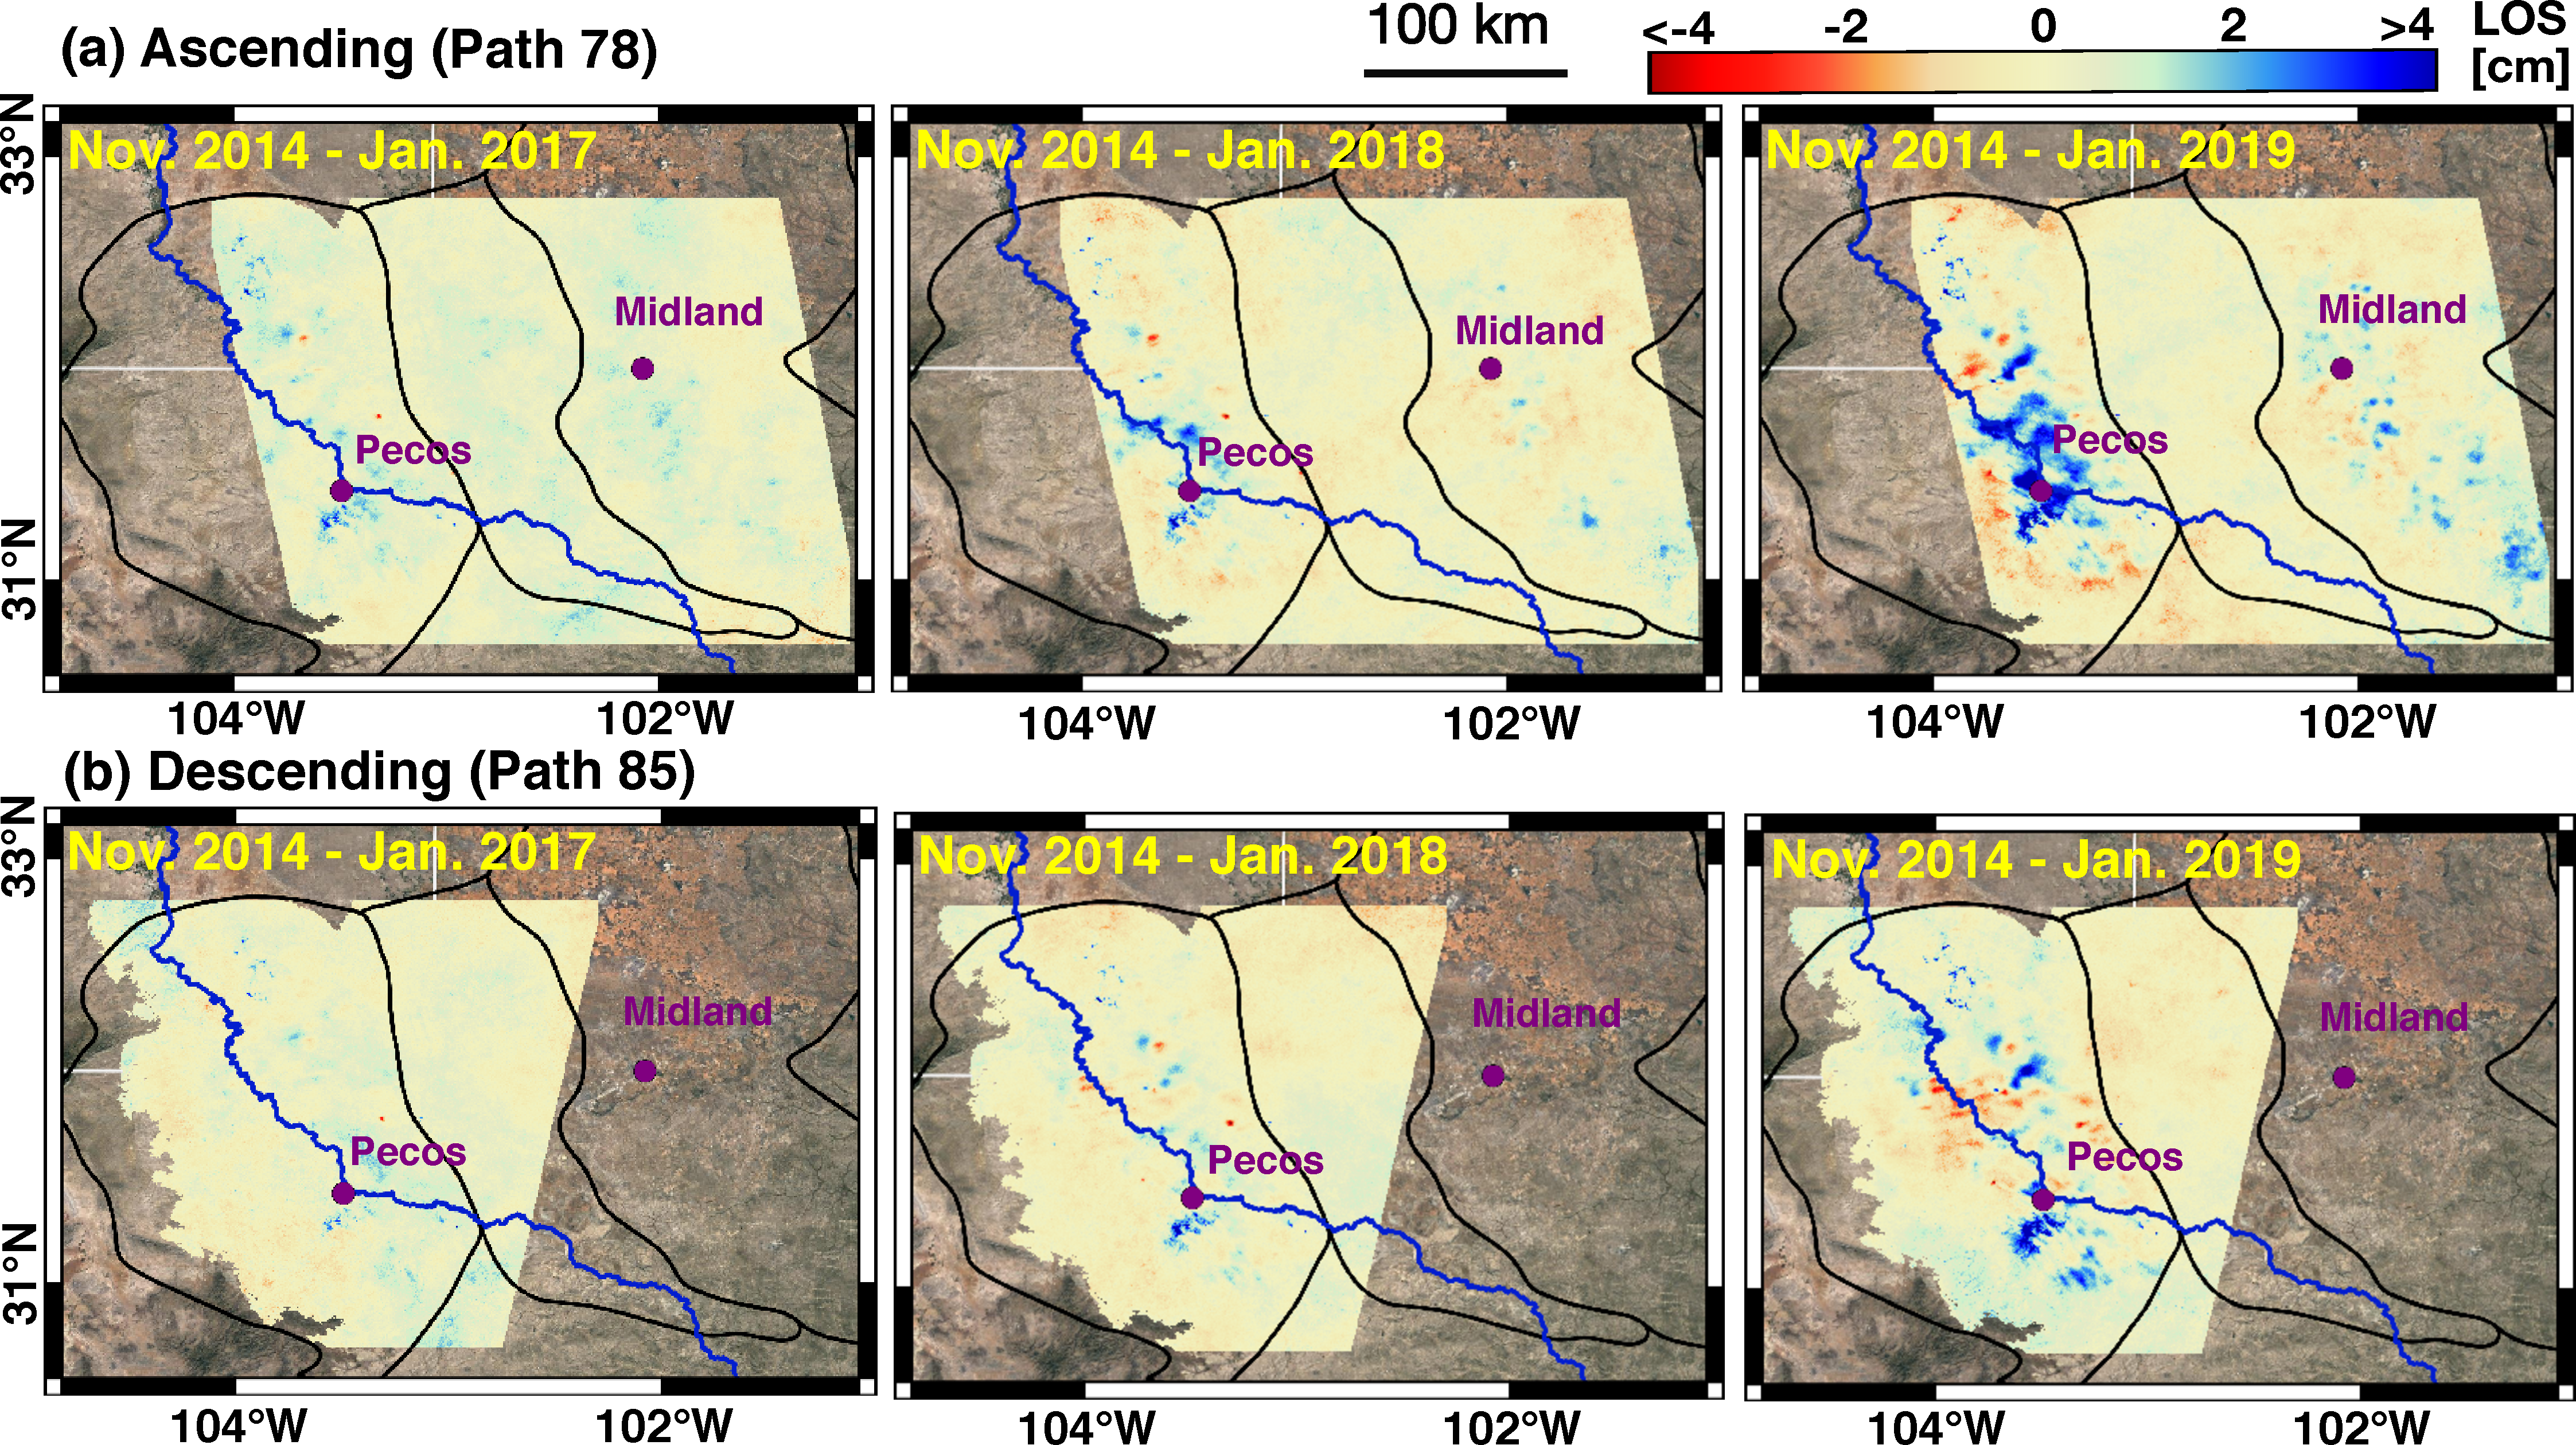
\includegraphics[width=.99\linewidth]{figures/chapter4-grl/figure3-los-insar.pdf}
	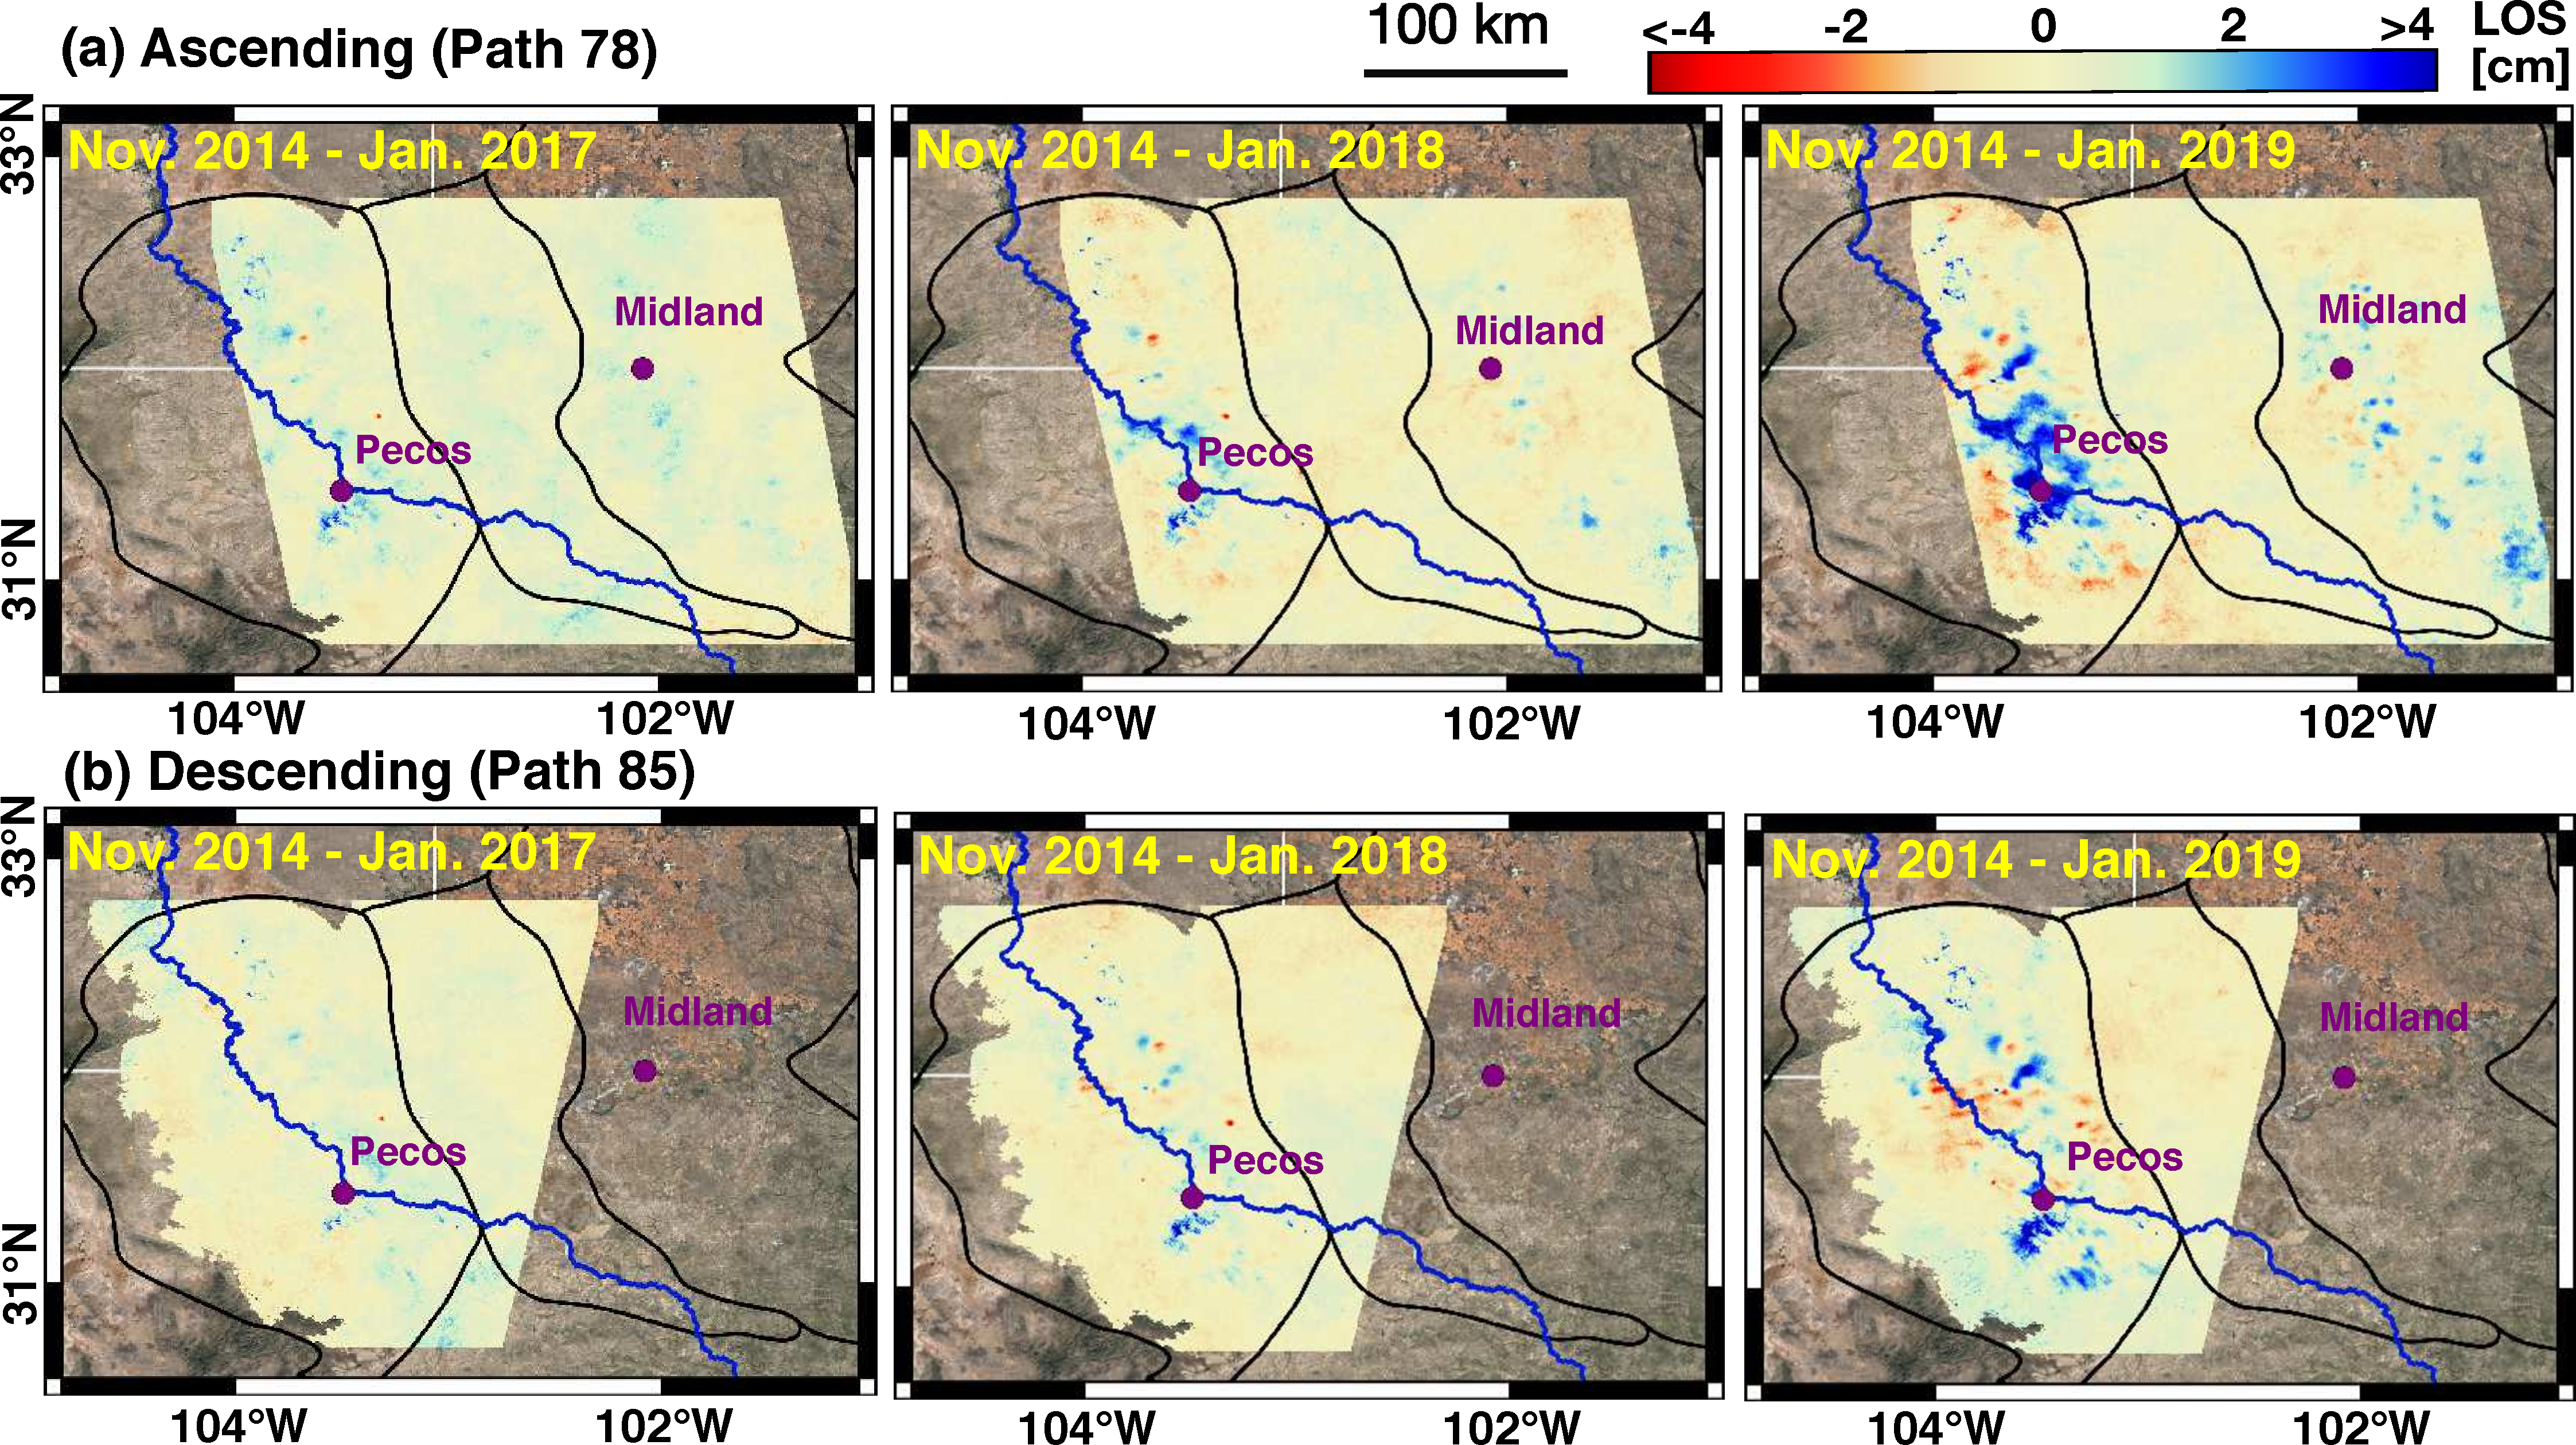
\includegraphics[width=.99\linewidth]{figures/chapter4-grl/figure3-los-insar-small.pdf}
	\caption[Cumulative LOS deformation for Path 78 and Path 85]{Cumulative LOS deformation (Nov. 2014 - Jan.2017; Nov. 2014 - Jan.2018; Nov. 2014 - Jan. 2019) as inferred from Sentinel-1 (a) ascending Path 78, and (b) descending Path 85 data over an 80,000 square km oil-producing region of the Permian Basin. Here a subsidence or eastward deformation signal leads to a positive LOS measurement in the ascending geometry, and a subsidence or westward deformation signal leads to a positive LOS measurement in the descending geometry. Areas with $>$1200 m altitude are masked due to the low oil production activity in mountainous regions.}
	\label{fig:ch4-insar-los}
\end{figure}



\begin{figure}
	\centering
	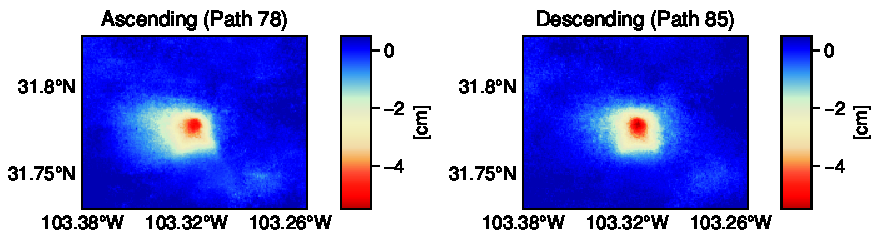
\includegraphics[width=\textwidth]{figures/chapter2-sar/injection-asc-desc.pdf}
	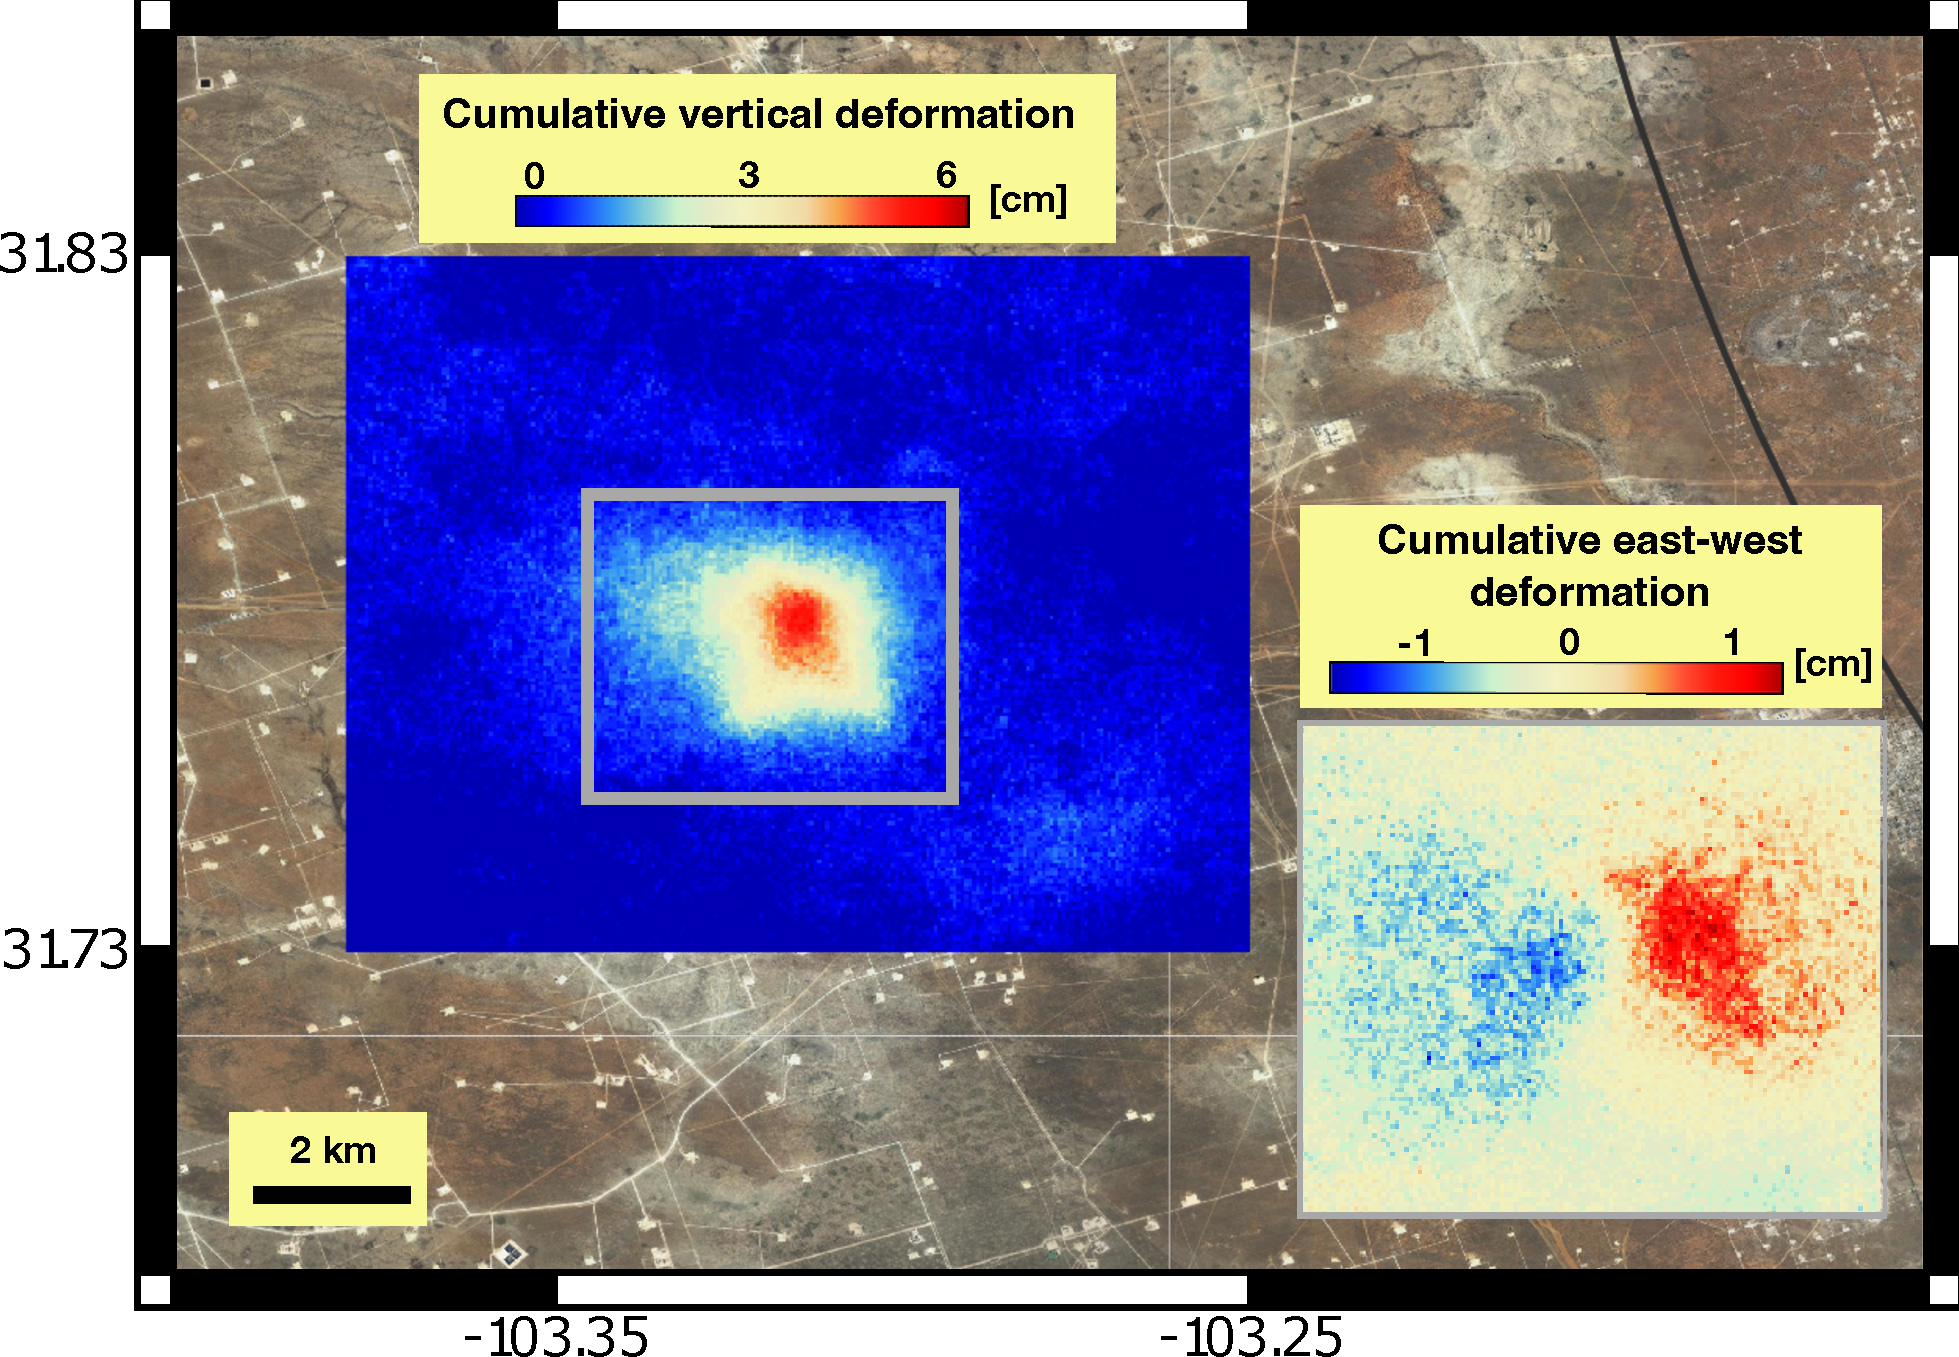
\includegraphics[width=\textwidth]{figures/chapter2-sar/injection-kim-lu}
	%	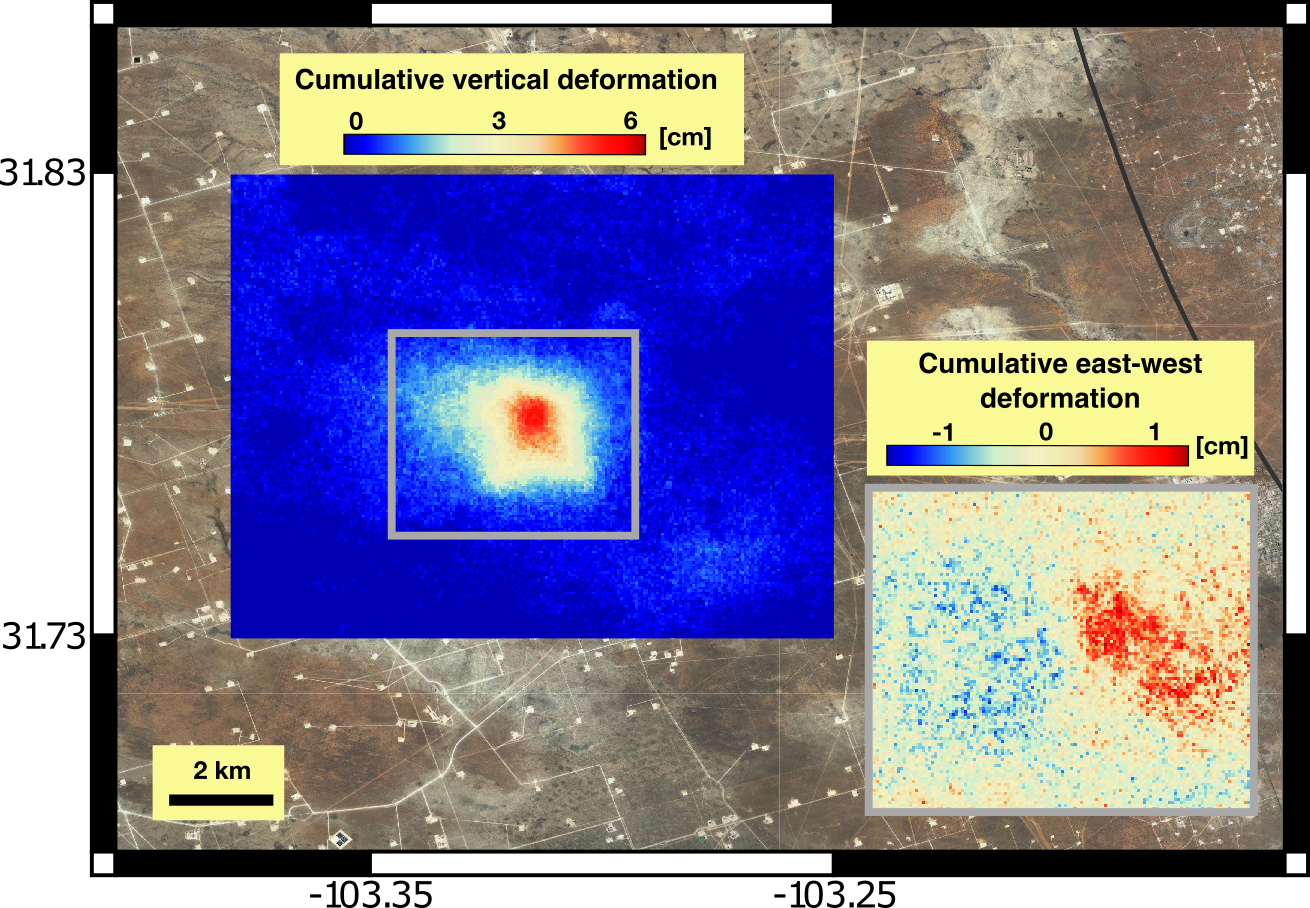
\includegraphics[width=\textwidth]{paper1-permian/figures/supplement/figureS3-injection-kim-lu.pdf}
	\caption[Vertical and horizontal deformation near Winkler County, TX]{
		(top) Ascending and descending line-of-sight cumulative deformation between November 2014 and April 2017. Red indicates motion toward each satellite.
		(bottom) Cumulative vertical and horizontal surface deformation due to wastewater injection in Winkler County, TX. The horizontal motion here is $\sim$ 20\% of the vertical motion, with up to $\sim$ 5.5 cm of uplift and $\sim$ 1.2 cm of east-west motion. This localized deformation feature was originally reported in \cite{Kim2018AssociationLocalizedGeohazards}.}
	\label{fig:ch2-injection-kim-lu}
\end{figure}


We also solved for the vertical and eastward deformation in the region where Path 78 and 85 overlap (see Section \ref{sec:ch4-insar-decomp}) using the LOS unit vector at each pixel location (Figure \ref{fig:los-map}).
%We decomposed the ascending and descending LOS solutions from Figure \ref{fig:ch4-insar-decomp} to find the horizontal and vertical deformation.
To illustrate the decomposition, Figure \ref{fig:ch2-injection-kim-lu} shows a 12 km x 12 km region centered on a wastewater injection well found by \cite{Kim2018AssociationLocalizedGeohazards} to have injection-related uplift. We observe similar magnitude deformation toward the satellite in both ascending and descending tracks (Figure \ref{fig:ch2-injection-kim-lu} top). 
%After decomposing the two geometries using the LOS vector at each pixel, 
After decomposing the two geometries, we calculated $\sim$ 5.5 cm of uplift and $\sim$1.2 cm of east-west motion between November 2014 and April 2017 (Figure \ref{fig:ch2-injection-kim-lu} bottom), similar to the magnitudes found in \cite{Kim2018AssociationLocalizedGeohazards}.

% ORIGINAL:  \cite{Kim2018AssociationLocalizedGeohazards} detected several localized deformation features within the Delaware Basin related to wastewater injection, CO2 injection, and hydrocarbon production using Sentinel-1 InSAR data.  Our LOS decomposition results are consistent with their study at these locations. For example, in a 12 km x 12 km region centered on a wastewater injection well, we observed $\sim$ 5.5 cm of uplift and $\sim$1.2 cm of east-west motion between November 2014 and April 2017 (Figure \ref{fig:injection-kim-lu}). 



In the northern Delaware Basin, where large volumes of oil production and wastewater disposal occurred, the ascending and descending LOS deformation patterns are similar. This means that the observed deformation in this region is primarily vertical (Figure \ref{fig:ch4-insar-decomp} (b) and (e)). The observed subsidence or uplift features between Nov. 2014 and Jan. 2019 are $\sim$ 1-4 cm. In the southern Delaware Basin, \cite{Deng2020SurfaceDeformationInduced} solved for the cumulative LOS surface deformation between Nov. 2014 and Feb. 2019 ($\sim$ 100 km by 60 km) using the ascending Sentinel-1 data (Path 78 frames 99-100). In this study, we found that the observed magnitudes of the ascending and descending LOS deformation are different (Figure \ref{fig:ch4-insar-los}), which suggests that both horizontal and vertical deformation occurred in this region. Previous studies near Mesquite, Nevada have shown that confined aquifer pumping in the presence of faults can produce complex asymmetrical deformation patterns with a non-trivial horizontal component \citep{Burbey2008InfluenceGeologicStructures}. In the Pecos area, the largest subsidence patterns ($\sim$ 13 cm over 4 years) occurred $\sim$ 15 km south of Pecos, and the largest eastward motion ($\sim$ 3-4 cm over 4 years) occurred near the town of Pecos along a line transect (Figure \ref{fig:ch4-insar-decomp} (c) and (f)). The observed linear deformation patterns align with the inferred favorable fault plane orientation proposed by \cite{LundSnee2018StateStressPermian} (a strike angle of $\sim$ 300 degrees, lining up with the measured $S_{Hmax}$ direction), and they also align with a cluster of recent shallow earthquakes ($<$ 3 km depth) cataloged by TexNet.



\begin{figure}
	\centering
	%	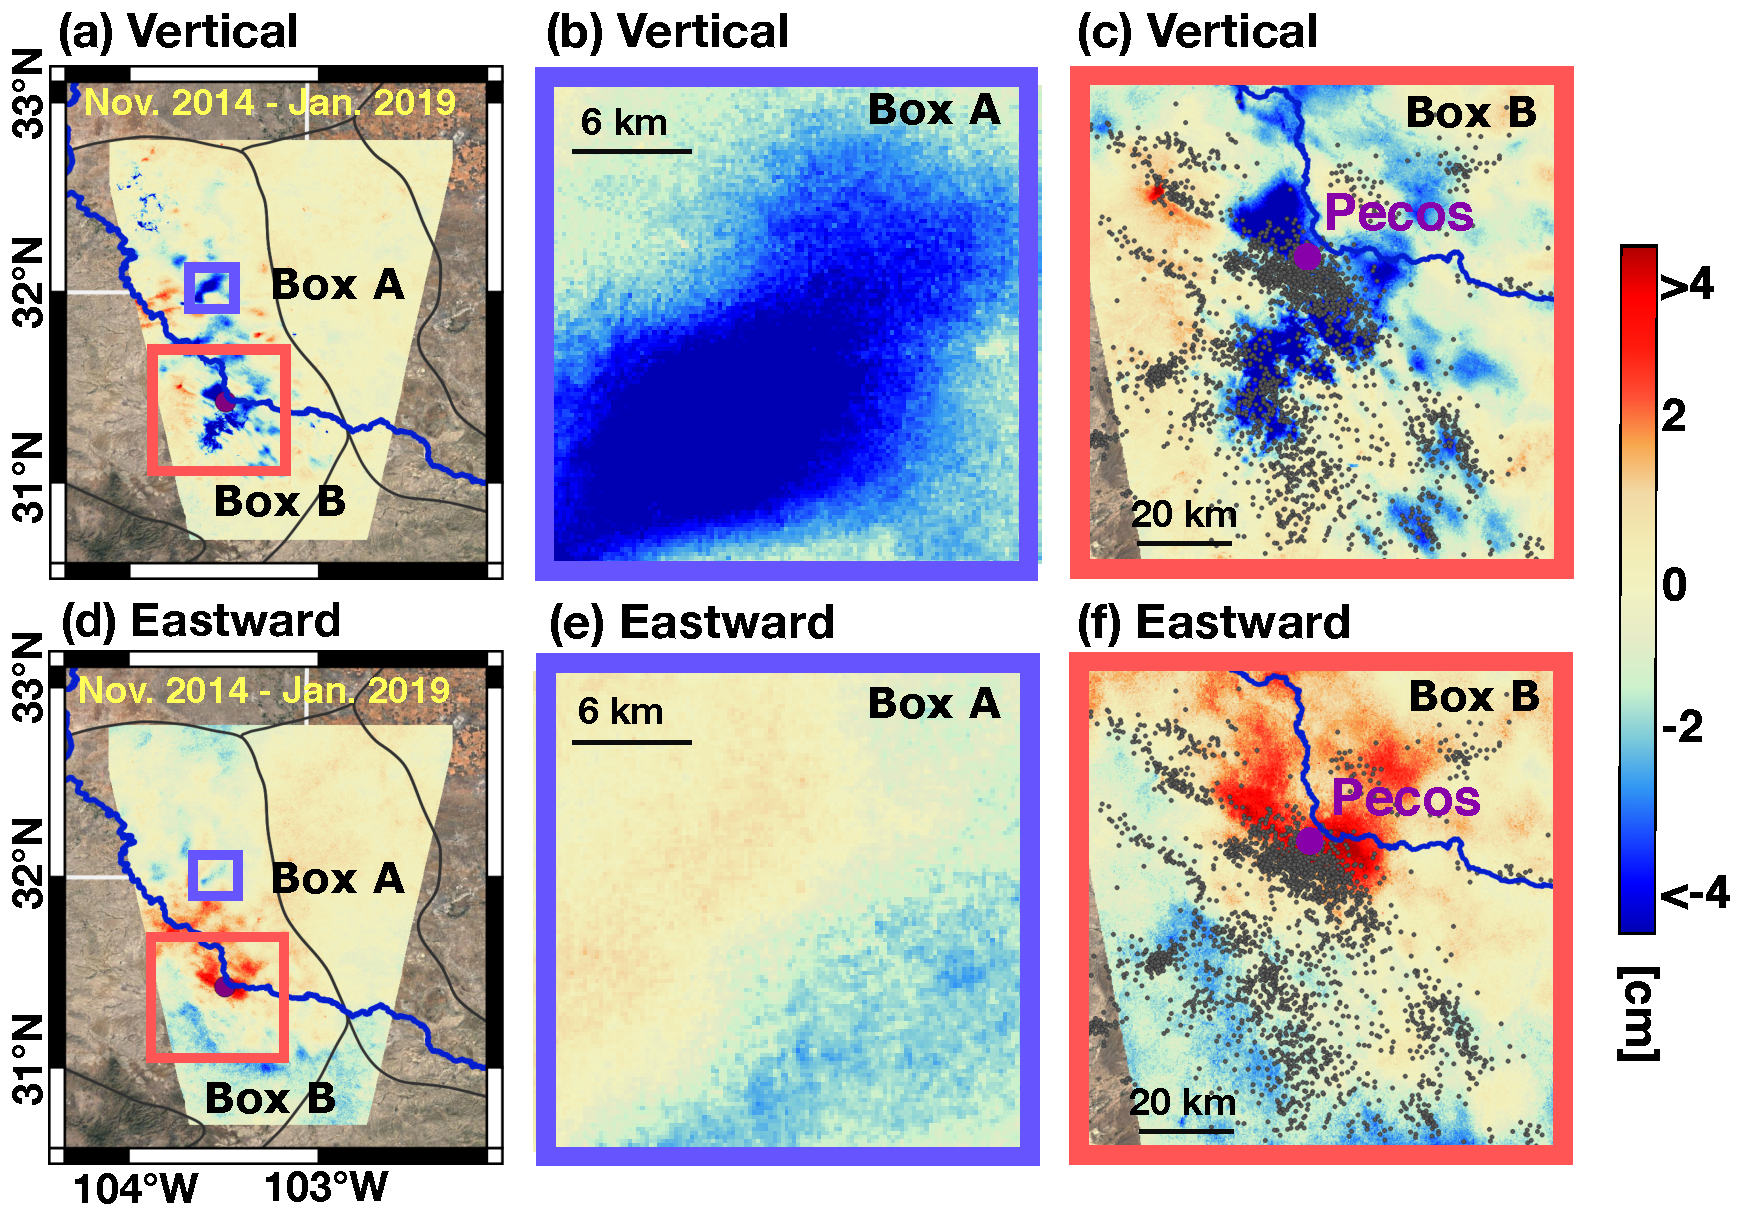
\includegraphics[width=0.96\linewidth]{figures/chapter4-grl/figure4-east-vertical-6panel-labelled.pdf}
	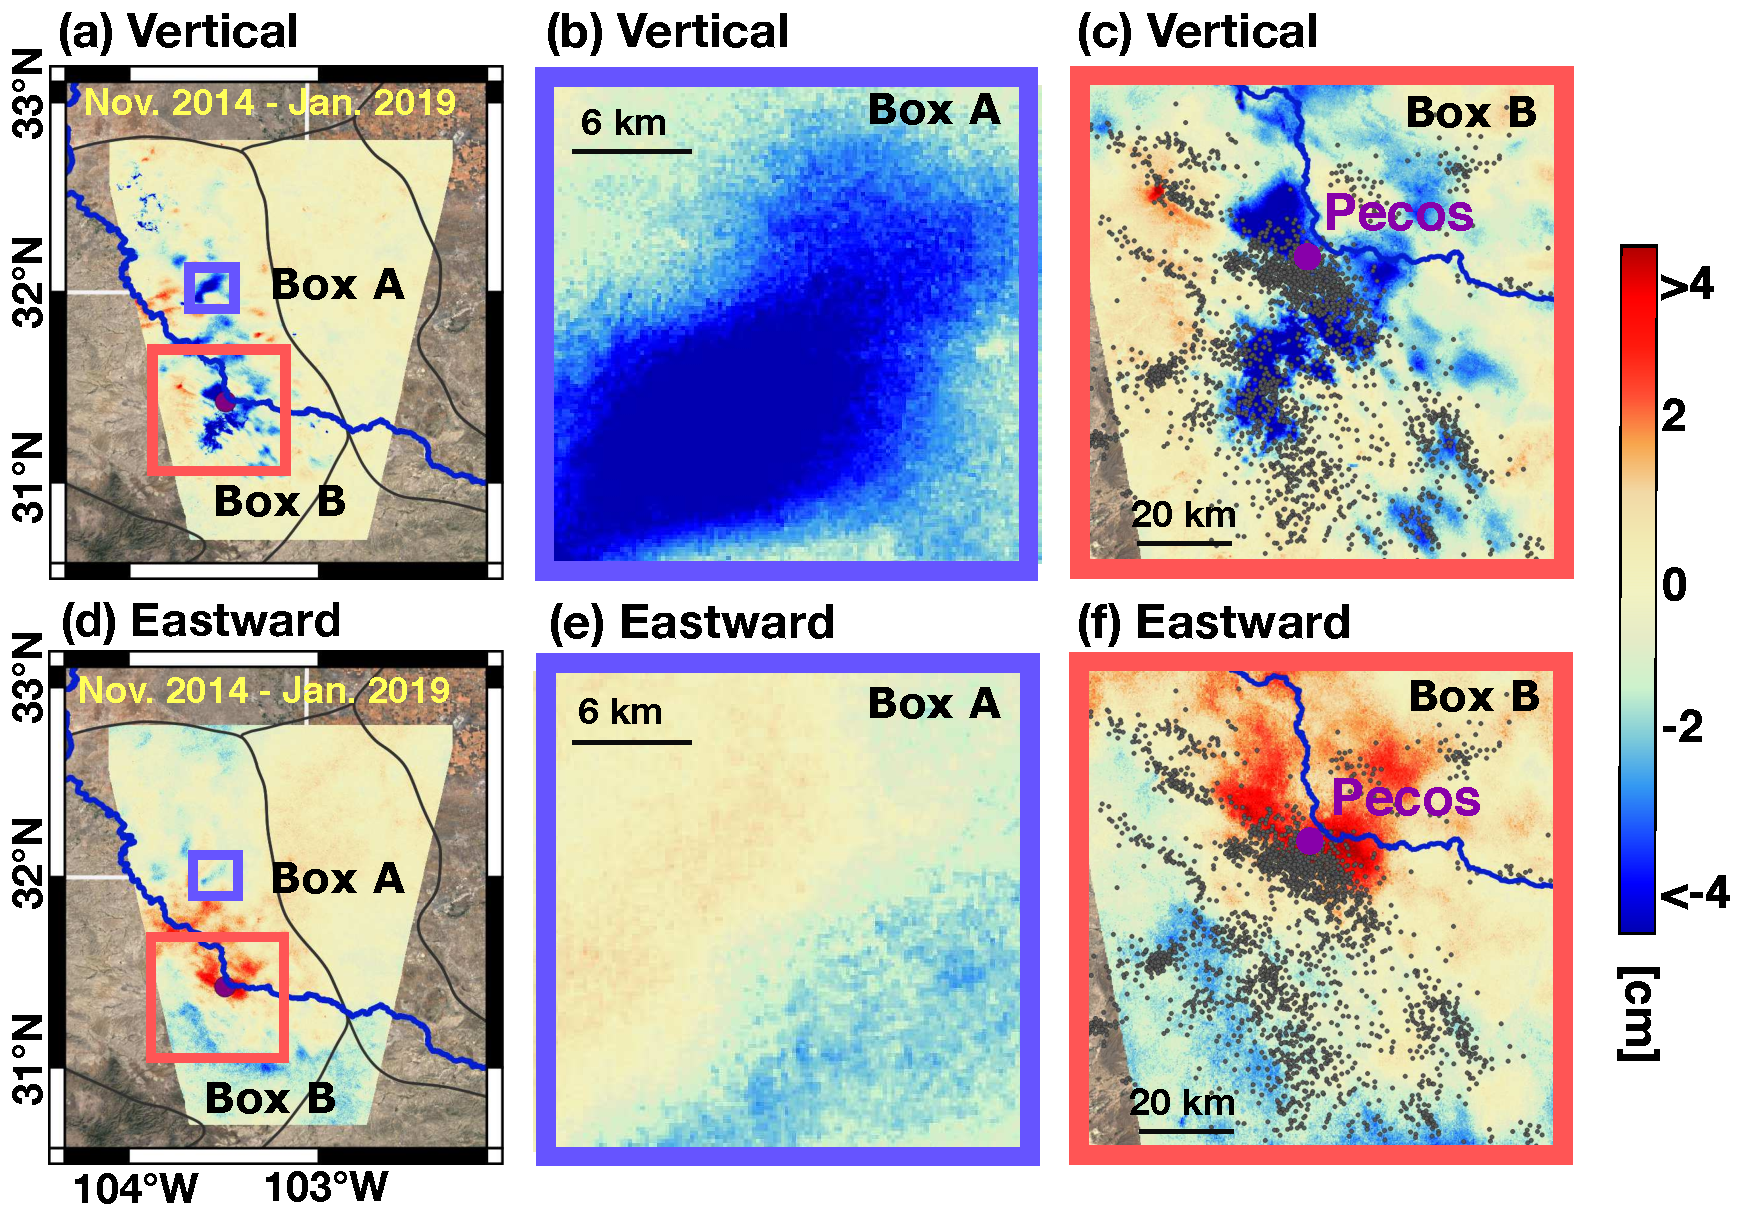
\includegraphics[width=0.96\linewidth]{figures/chapter4-grl/figure4-east-vertical-6panel-labelled-small.pdf}
	\caption[Cumulative vertical and horizontal deformation]{(a) Cumulative vertical deformation between Nov. 2014 and Jan. 2019 over the region where Sentinel-1 Path 78 and Path 85 overlap. A zoomed-in view of Box A in the northern Delaware Basin and Box B in the southern Delaware Basin are shown in panel (b) and (c) respectively. (d) Cumulative eastward deformation between Nov. 2014 and Jan. 2019 over the region where Sentinel-1 Path 78 and Path 85 overlap. A zoomed-in view of Box A in the northern Delaware Basin and Box B in the southern Delaware Basin are shown in panel (e) and (f) respectively. In the southern Delaware Basin, the observed vertical and eastward deformation (panel (c) and (f)) show linear patterns along with earthquake hypocenters (gray dots) detected by TexNet in 2018.}
	\label{fig:ch4-insar-decomp}
\end{figure}

\FloatBarrier

\section{Implications for geomechanical modeling}
Based on fault plane solutions derived from recent seismic activity and the faulting stress regime interpretations \citep{LundSnee2018StateStressPermian}, the Pecos area is in a normal faulting regime. We employed an elastic dislocation model \citep{Okada1992InternalDeformationDue} to demonstrate that the presence of dip-slip normal faults can produce the observed linear subsidence patterns in this area (Figure \ref{fig:ch4-model} (a)). We solved for the dip angle, depth, width along the dip direction, and slip magnitude of four normal faults by best fitting the forward model to InSAR vertical deformation observations, minimizing the sum of squared residuals, and maximizing the r-squared values \citep{Du1992ComparisonVariousInversion} (Appendix \ref{appen:okada}). The optimal solution suggests that the depth of the faults ranges from 0.9 km to 1.5 km, which is shallower than most of the TexNet recorded earthquakes (2-6 km in depth). Possible explanations for this discrepancy include: (1) the existence of aseismic fault slippage being responsible for the observed surface deformation \citep{McGarr2017WastewaterDisposalEarthquake}; (2) bias in earthquake depth estimation in the TexNet catalog \citep{Lomax2019ImprovingAbsoluteEarthquake}; (3) systematic modeling errors associated with representing a mechanically layered earth as a homogeneous half space \citep{Du1992ComparisonVariousInversion}. 



\begin{figure}
	\centering
	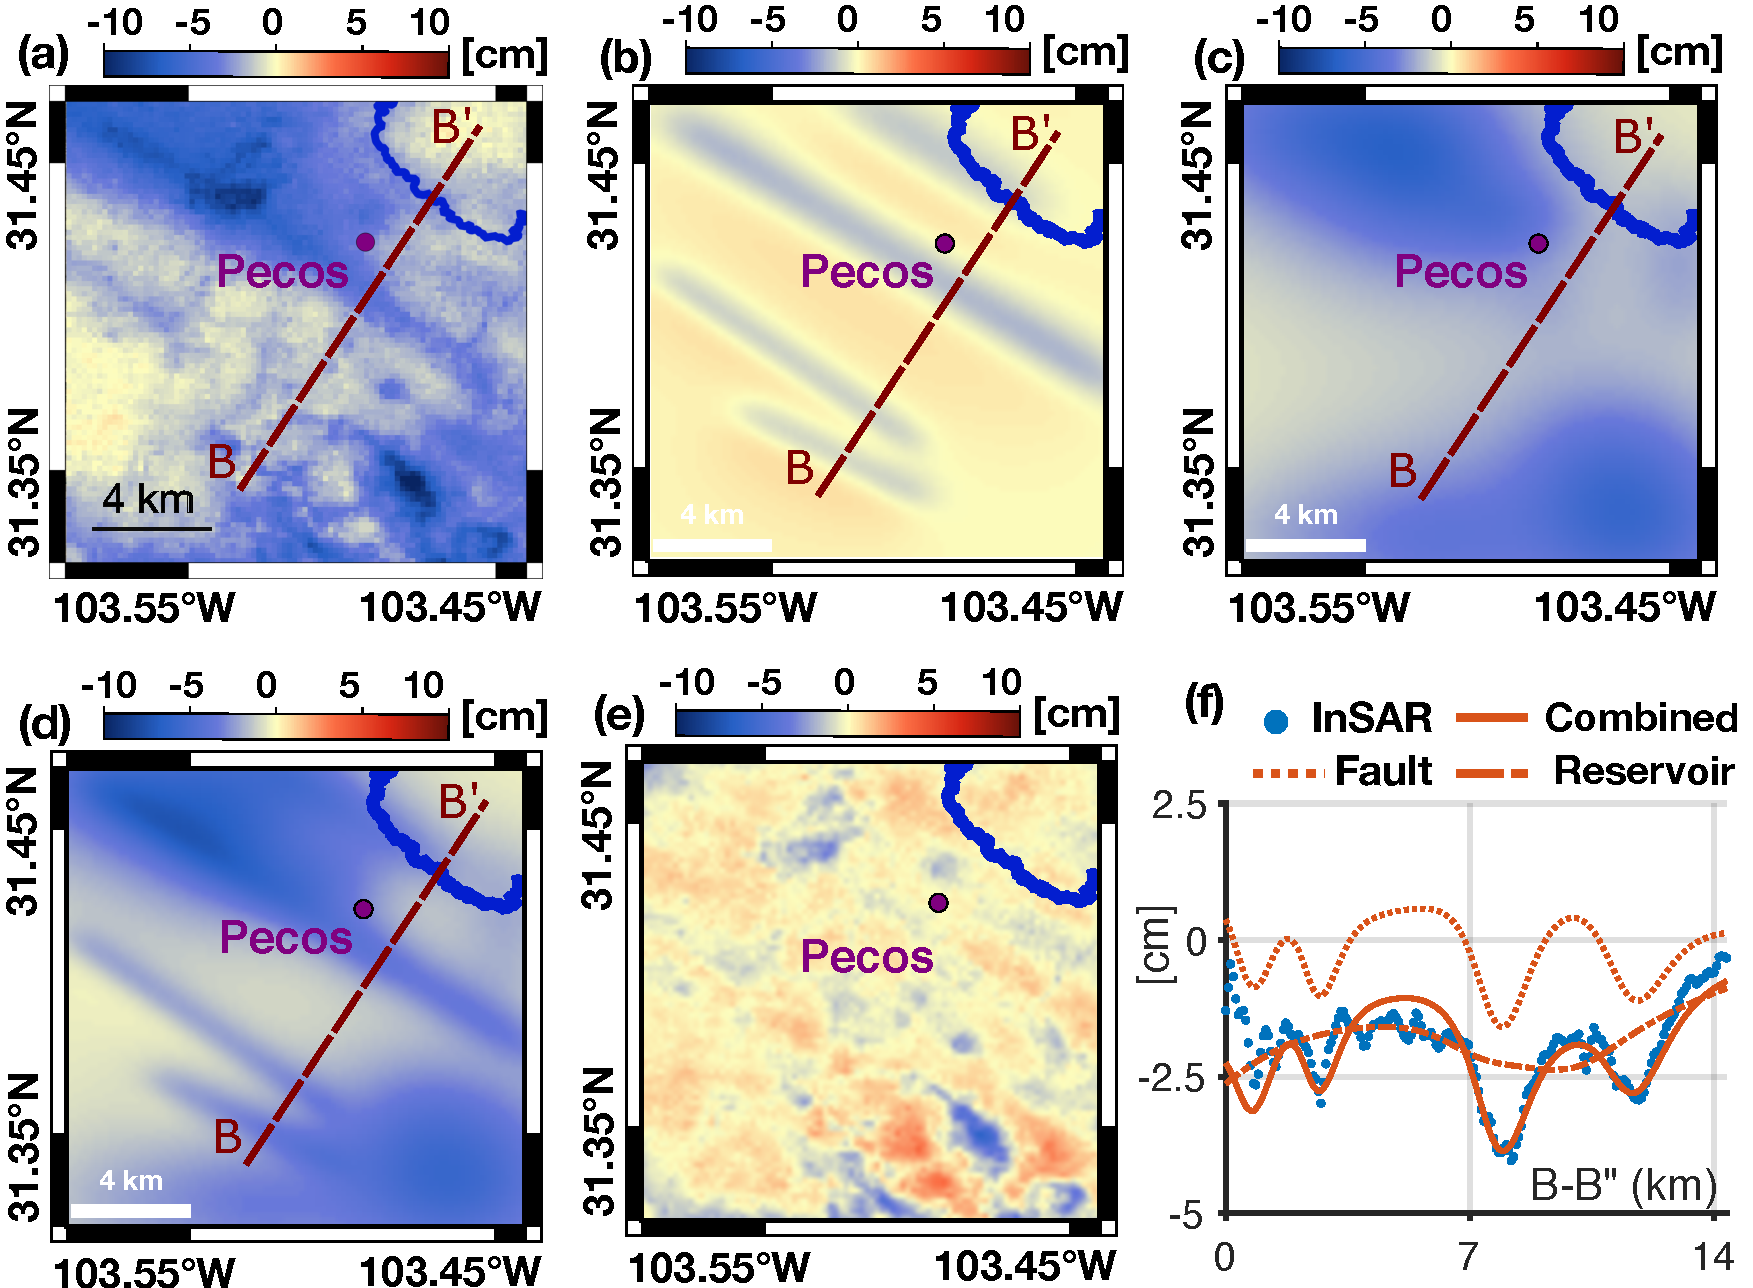
\includegraphics[width=\linewidth]{figures/chapter4-grl/figure5-modeling.pdf}
	\caption[Modeled surface deformation from fault slip and reservoir subsidence]{(a) InSAR-observed cumulative vertical deformation between Nov. 2014 and Jan. 2019 in the Pecos, TX area. (b) Modeled vertical deformation associated with four dip-slip faults. (c) Modeled vertical deformation associated with reservoir compaction. (d) Modeled total vertical deformation associated with four dip-slip faults and reservoir compaction (panel (b) $+$ panel (c)). (e) Difference between InSAR-observed and model-predicted vertical deformation (panel (a) $-$ panel (d)). (f) Difference between InSAR-observed and model-predicted vertical deformation along the B-B' transect.}
	\label{fig:ch4-model}
\end{figure}


After removing the best-fit deformation associated with dip-slip faulting (Figure \ref{fig:ch4-model} (b)), there is still $\sim$ 2 cm residual subsidence in the Pecos area (e.g. Figure \ref{fig:ch4-model} (f)). Given that shallow groundwater production was minimal in this region for the time period of interest \citep{Deng2020SurfaceDeformationInduced}, we introduced an elastic reservoir compaction model \citep{Geertsma1973LandSubsidenceCompacting} to our geomechanical analysis (Appendix \ref{appen:model-compact}). We implemented two layers of multiple cylindrical reservoirs corresponding to reported locations and depths of well clusters in the Delaware Mountain Group (DMG) and Wolfcamp reservoirs, which account for most of the recent oil and gas production in the region. We discretized the DMG layer based on a cluster of production wells predominantly perforated over a depth range of 1.5-1.8 km. The Wolfcamp wells are completed over a depth range of 3-3.6 km. We employed an objective function inversion method to solve for the reservoir pressure depletion pattern that best fit the InSAR-observed subsidence (Figure \ref{fig:ch4-model} (c)) \citep{Du2001PoroelasticReservoirModel}.

An important conclusion of this study is that both fault slip and reservoir inflation or compaction can produce observable surface deformation over an 80,000 square kilometer oil-producing region of the Permian Basin. The InSAR-observed subsidence patterns over the Pecos area can be modeled as slip over multiple faults and discretized cylindrical reservoir compaction (Figure \ref{fig:ch4-model} (d)-(f)). We note that InSAR subsidence data alone can constrain all pertinent fault and reservoir parameters in our normal faulting and reservoir compaction models. The InSAR observed cumulative surface deformation patterns, which show larger horizontal component than the model prediction, suggest that other factors, such as strike-slip faulting and heterogeneity in subsurface properties, may play a role. There have been extensive studies on how reservoir compaction and inflation as well as fault slippage alter stress fields in the subsurface and produce surface deformation \citep{Geertsma1973LandSubsidenceCompacting,Segall1992InducedStressesDue,Okada1992InternalDeformationDue,Du1992ComparisonVariousInversion,Vasco2005UseQuasiStatic,Vasco2008ReservoirMonitoringCharacterization,Khakim2012GeomechanicalModelingInsar}. InSAR surface deformation can be combined with this knowledge to evaluate fluid recovery efficiency and monitor disposal wells at low cost. Furthermore, these high-quality geodetic measurements are readily available to complement the TexNet seismic catalog for assessing the likelihood of fault motion and induced earthquake risks in Texas.


